\documentclass[utf8x]{ctexart}
\usepackage{setspace}
\usepackage{url}
\onehalfspacing
\usepackage{amsmath,amssymb,amsfonts,amsthm,mathtools}
\usepackage[english]{babel}
\usepackage[T1]{fontenc}
\usepackage{lmodern}
\usepackage{dsfont}
\usepackage{bbm}
\usepackage[round]{natbib}
\usepackage{color} 
\usepackage[defaultlines=2,all]{nowidow}
\usepackage{caption}
\usepackage[labelformat=simple]{subcaption}
\usepackage{makecell}
\renewcommand\thesubfigure{(\alph{subfigure})}

\setlength\parindent{0pt}
\setlength{\parskip}{6pt plus 1pt minus 1pt}

\newcommand{\red}{\textcolor{red}}


\begin{document}

\begin{titlepage}
  \centering
  {\scshape\LARGE National Taiwan University \par}
  \vspace{1cm}
  {\scshape\Large Financial Technology \par}
  \vspace{2cm}
  {\huge\bfseries Project 3: Push Notification Click Prediction\par}
  \vspace{2cm}
  {\Large Lecturer:\\
    Che Lin (林澤) \par}
  \vspace{1cm}
  {\Large Author: Tadeo Hepperle, Student ID: A11922105 \par}
  \vfill
  {\large \today\par}
\end{titlepage}


\tableofcontents

\cleardoublepage

\section{Introduction}

In this project we will attempt to use bidirectional LSTMs, GRUs and a Transformer Encoder model to predict if a push notification will be clicked. As input, we give to the model information about the past 10 push notifications that have been sent out to the user that receives the current push notification, including the day of the week and the topic of each notification.
The models are trained on the binary response whether a push notification is clicked or not and are expected to give good binary predictions on unseen data.

\subsection{Description of the Data}

The data for the project was provided by the "AviviD Innovative Media" company, that excels in digital marketing. There are 150023 push notifications in the data, that were sent to 1427 different users. This amounts to about 100 push notifications per user that have been sent over a period of 10 days, so roughly 10 push notifications per day. Each push notification represents a news from one of 19 categories, that include a wide range of topics. Examples for such topics are: "Technology", "Games", "Politics" and "China". All of these topics are one-hot-encoded. The respective weekday has also been one-hot-encoded, because it might be an important predictor. Together, weekday and topic form a 27-element binary vector for each push notification. The data has been aggregated to include a 11x27 matrix for each notification, representing the features of this push notification and the 10 that have been most recently sent to the same user. This allows us to utilize sequential models such as LSTM and GRU for the predictions.
For push notifications early on in a user's history, where less than 10 previous notifications are available, the first few rows of the 11x27 matrix have been padded with zero-values.

\subsubsection{Splitting the Data}

The data was split into 3 parts along the time axis:
\begin{itemize}
  \item Train set: 2022/08/01-2022/08/07, 105320 items
  \item Validation set: 2022/08/08-2022/08/09, 34362 items
  \item Test set: 2022/08/10, 10341 items
\end{itemize}
The data is fairly imbalanced, with only 1519 of the 150023 items being clicks (label=1). This is just 1.01\% and could lead models to ignore the minority class. The 148504 remaining cases were all either ignored by the user or blocked.

\subsection{Description of Methods}

To predict whether a push notification is clicked we use bi-directional LSTMs, GRUs and a Transformer Encoder Layer.
All of these models follow the same principle: encode a $k$-dimensional input vector over $t$ time steps into an $e$-dimensional encoding. A linear combination of all $e$ elements of the $e$-dimensional encoding vector is then produced by a linear fully connected layer to produce a single scalar output. This scalar is then transformed by a sigmoid function to produce values between 0 and 1, which can be interpreted as predicted click-probabilities.

\subsubsection{Loss Function and Optimizer}

The binary cross entropy loss (BCE) has been used as a criterion for the gradient descent in training:
\[ BCE = -(y\log{1-p}+(1-y)\log{1-p}) \]
To optimize the models, the Adam optimizer with a learning rate of 0.001 has been utilized throughout the report. Other learning rates were tried but were either too slow to converge or were too high and therefore too "jumpy" and could not get the error low enough consistently. A batch size of 256 was used in training.

\subsubsection{Bi-Directional LSTM}

A unidirectional LSTM, as described in the last report, just looks at past data and updates the hidden state and cell state in each time step. In comparison, a bidirectional LSTM just consists of two unidirectional LSTMs, where one iterates over the time steps in a forward manner like the normal LSTM from 0 to $t$ and the other one learns by looking at the date from the back to the front, from time step $t$ to 0.
Each of them has a $hidden\_size$-dimensional cell state and hidden state respectively. The final encoding of the input sequence after consuming all time steps in their respective directions is then just a concatenation of the final hidden states of forward and backward LSTM. This is a vector of size  $2*hidden\_size$. Even though in principle a BiLSTM with a hidden size of $hidden\_size$ is not more powerful than a single LSTM with a hidden size of $2*hidden\_size$, in practice BiLSTM seem to learn a good representation of the data faster.

\subsubsection{Bi-Directional GRU}

A bidirectional general recurrent unit (BiGRU) relates to a unidirectional GRU in the same way a BiLSTM relates to an LSTM. only the implementation details in the two submodels (forward and backward) differ: the two GRUs used do not have a cell state like an LSTM cell and are less complicated to compute. How outputs are combined and predictions are made does not differ though. The BiGRU is like the BiLSTM parameterized by $hidden\_size$
For this paper we only trained single layer BiGRUs and BiLSTMs.
Implementation of the forward pass of our BiLSTM  and BiGRU in pytorch is displayed in Figure~\ref{fig:forwardpasses1}

\begin{figure}[htb]
  \centering
  \begin{subfigure}[b]{0.48\textwidth}
    \centering
    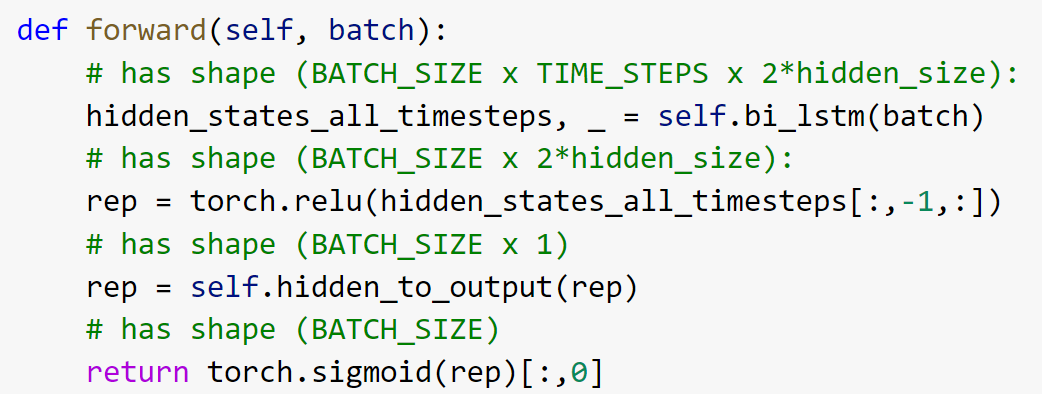
\includegraphics[width=\textwidth]{../images/forward_pass_lstm.png}
    \caption{Forward Pass BiLSTM}
    \label{fig:forwardpasses1_lstm}
  \end{subfigure}
  \begin{subfigure}[b]{0.48\textwidth}
    \centering
    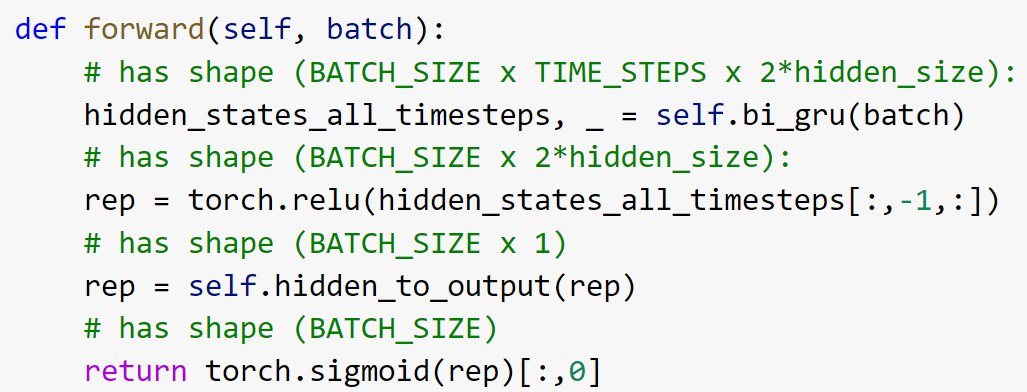
\includegraphics[width=\textwidth]{../images/forward_pass_gru.png}
    \caption{Forward Pass BiGRU}
    \label{fig:forwardpasses1_gru}
  \end{subfigure}
  \caption{Forward pass of BiLSTM and BiGRU are almost identical}
  \label{fig:forwardpasses1}
\end{figure}


\subsubsection{Transformer Encoder Layer}

A Transformer Encoder Layer (TEL) is one part of the popular Transformer-Architecture. It consists of a self-attention mechanism and a feed-forward layer. The output of the feed-forward layer can be mapped back to the input dimension to create an encoding that is hopefully better suited to be used in a linear prediction of a scalar value as the output. There are a number of attention heads that learn independently which parts of the input sequence are most important. In our implementation a feed-forward dimension of 64 has been chosen, we use 3 attention heads.

\section{Results}

We discovered that the loss of all models  starts to show signs of overfitting after the first 3-10 epochs. This effect is shown in Figure~\ref{fig:overfitting} where we trained a BiGRU with a hidden size of 64 for 100 epochs.

\begin{figure}[htb]
  \centering
  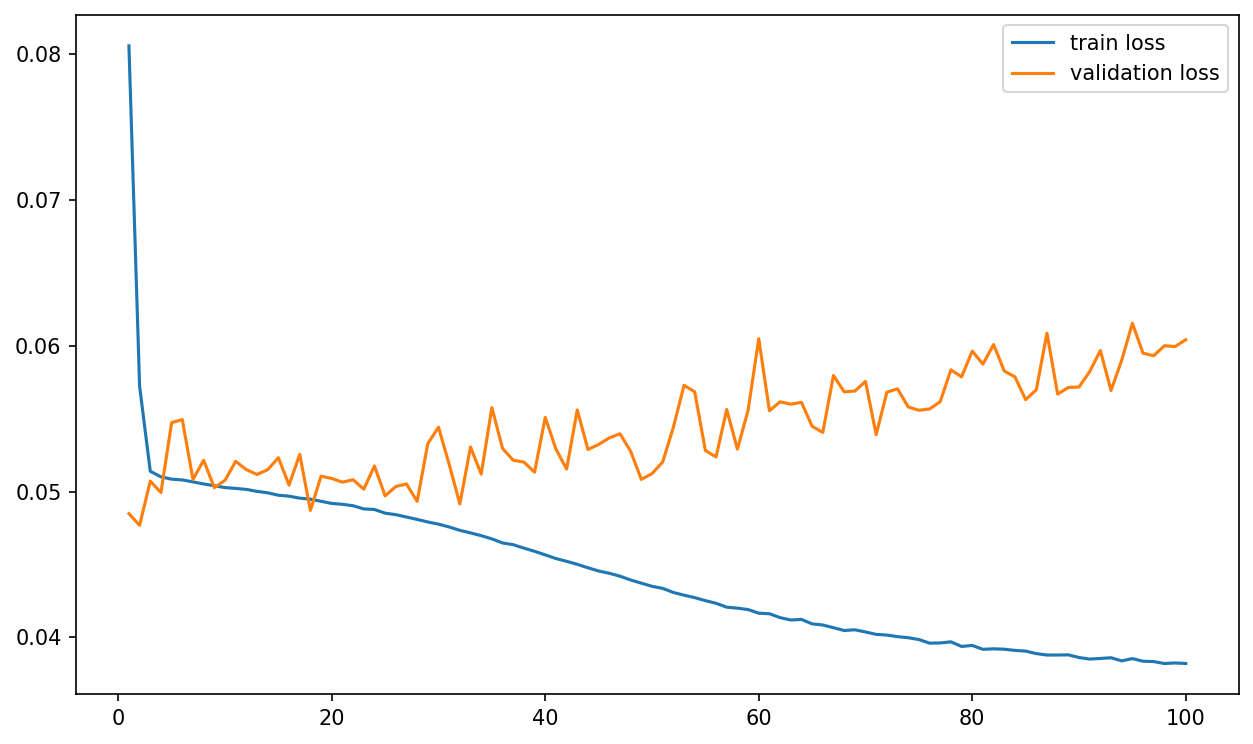
\includegraphics[width=\textwidth]{../images/BiGRU100_trainlosses.png}
  \caption{Overfitting behavior of a BiGRU with $hidden\_size = 64$}
  \label{fig:overfitting}
\end{figure}




Therefore, we choose to train our models for 10 epochs only and all statistics below are subject to this value. By experimentation a hidden size of 64 was chosen for the BiLSTM and BiGRU models.
Figure~\ref{fig:losses1} shows training and validation losses after training the BiLSTM, BiGRU and TEL models for 10 epochs. As we can see all models reach a test and train error of around 0.05. Table~\ref{tab:accuracy} displays the accuracy of the 3 models on train, validation and test set each.


\begin{figure}[htb]
  \centering
  \begin{subfigure}[b]{0.48\textwidth}
    \centering
    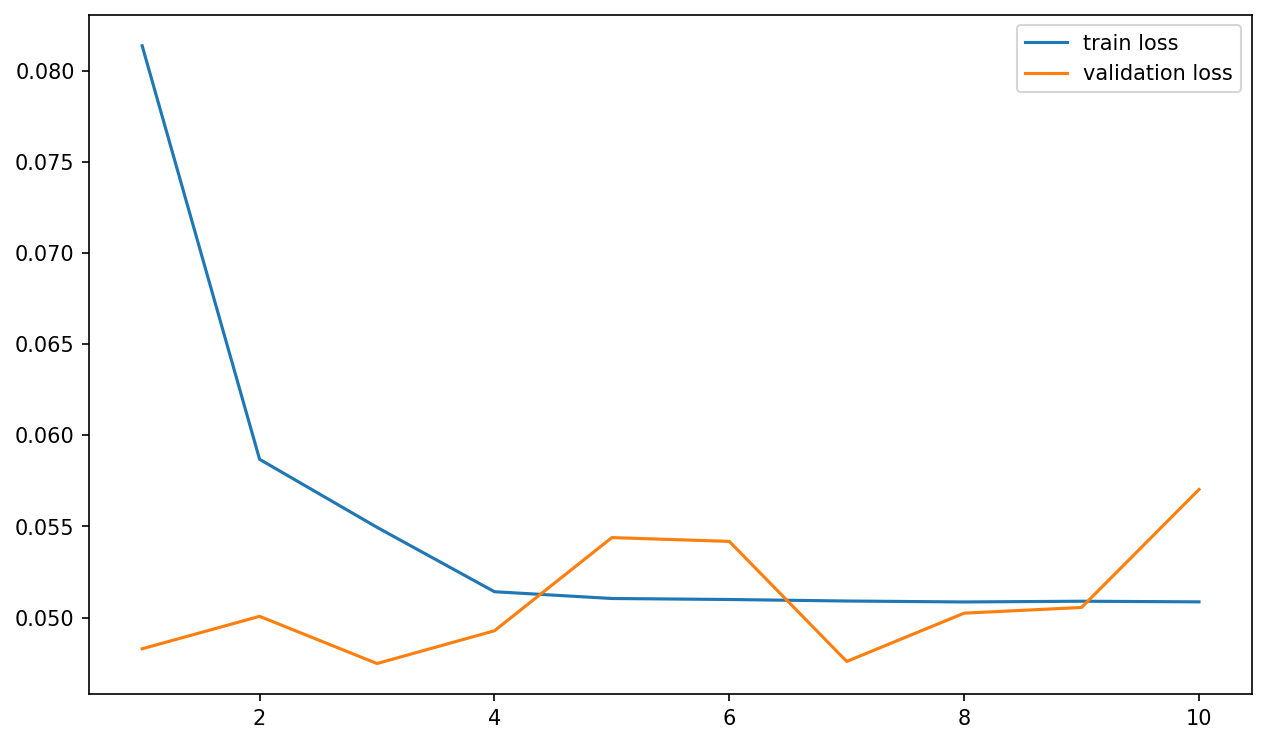
\includegraphics[width=\textwidth]{../images/BiLSTM_trainlosses.png}
    \caption{Train and Validation Loss BiLSTM}
    \label{fig:BiLSTM_trainlosses}
  \end{subfigure}
  \begin{subfigure}[b]{0.48\textwidth}
    \centering
    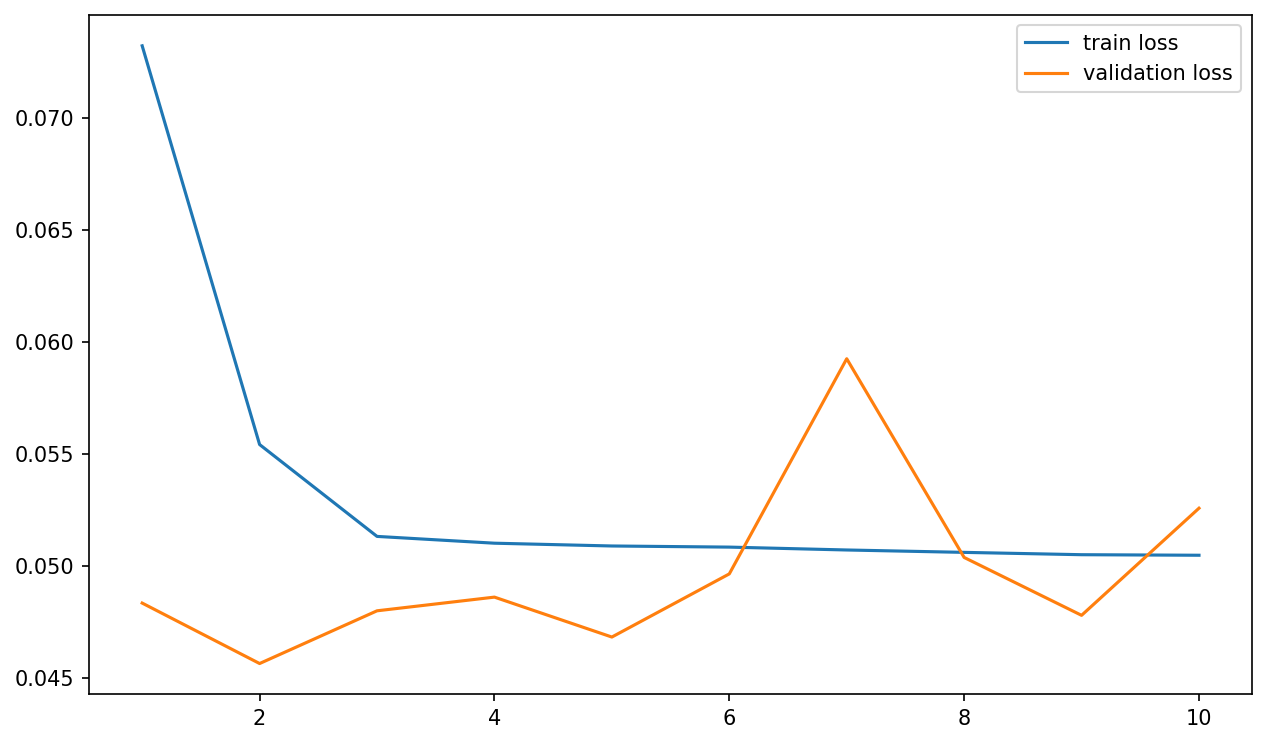
\includegraphics[width=\textwidth]{../images/BiGRU_trainlosses.png}
    \caption{Train and Validation Loss GRU}
    \label{fig:BiGRU_trainlosses}
  \end{subfigure}
  \begin{subfigure}[b]{0.48\textwidth}
    \centering
    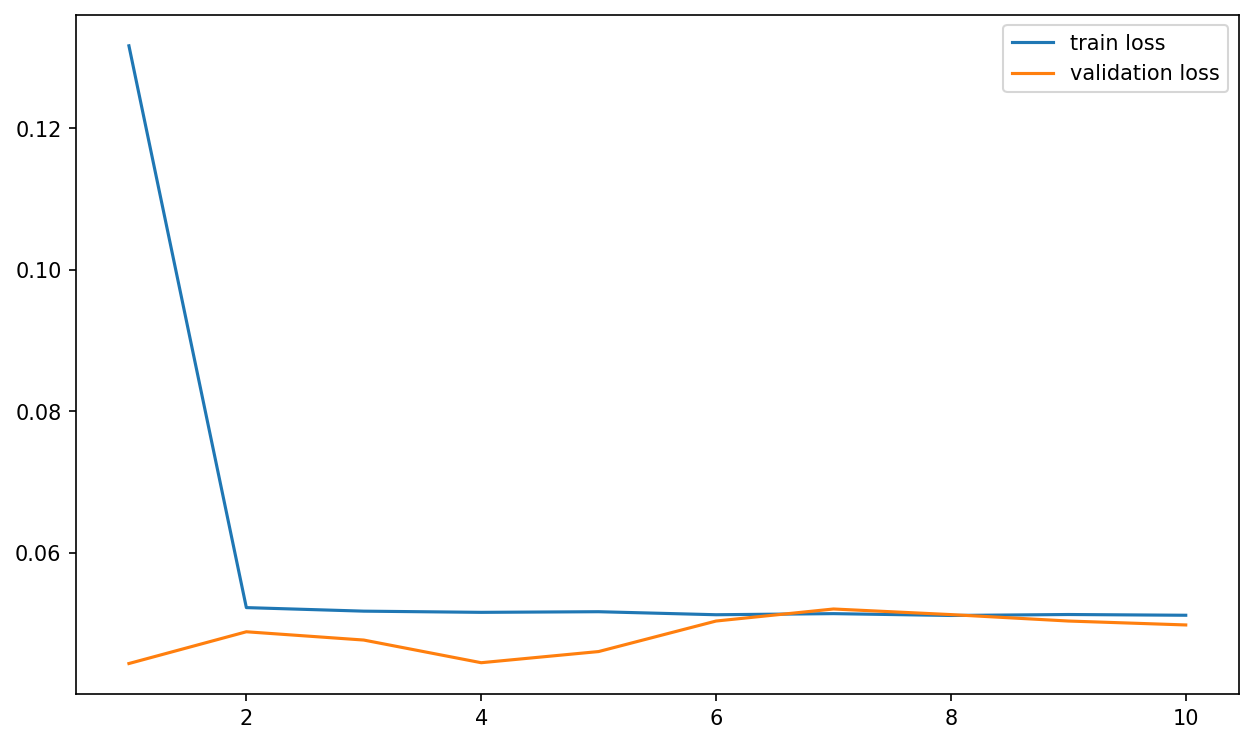
\includegraphics[width=\textwidth]{../images/Transformer_trainlosses.png}
    \caption{Train and Validation Loss Transformer Encoder Layer}
    \label{fig:TEL_trainlosses}
  \end{subfigure}
  \caption{Train and Validation Losses for all 3 models}
  \label{fig:losses1}
\end{figure}



\begin{table}[ht]
  \centering
  \caption{Accuracy of the 3 models}
  \label{tab:accuracy}
  \begin{tabular}{c|cccc}
    Accuracy & Train   & Validation & Test  \\
    \hline
    BiLSTM   & 0.989   & 0.992      & 0.989 \\
    BiGRU    & 0.00103 & 0.992      & 0.989 \\
    TEL      & 0.989   & 0.992      & 0.989 \\
  \end{tabular}
\end{table}


At a first glance the values in Table~\ref{tab:accuracy} seem very good. Such a high accuracy! But taking a closer look at the confusion matrices for all models, see Fig~\ref{fig:confusion} reveals that all models just predict "no click" for every single instance in every single set. This is likely an artifact of the imbalance of the data and should probably be dealt with by choosing a different loss function or an under/oversampling approach.


\begin{figure}[htb]
  \centering
  \begin{subfigure}[b]{0.32\textwidth}
    \centering
    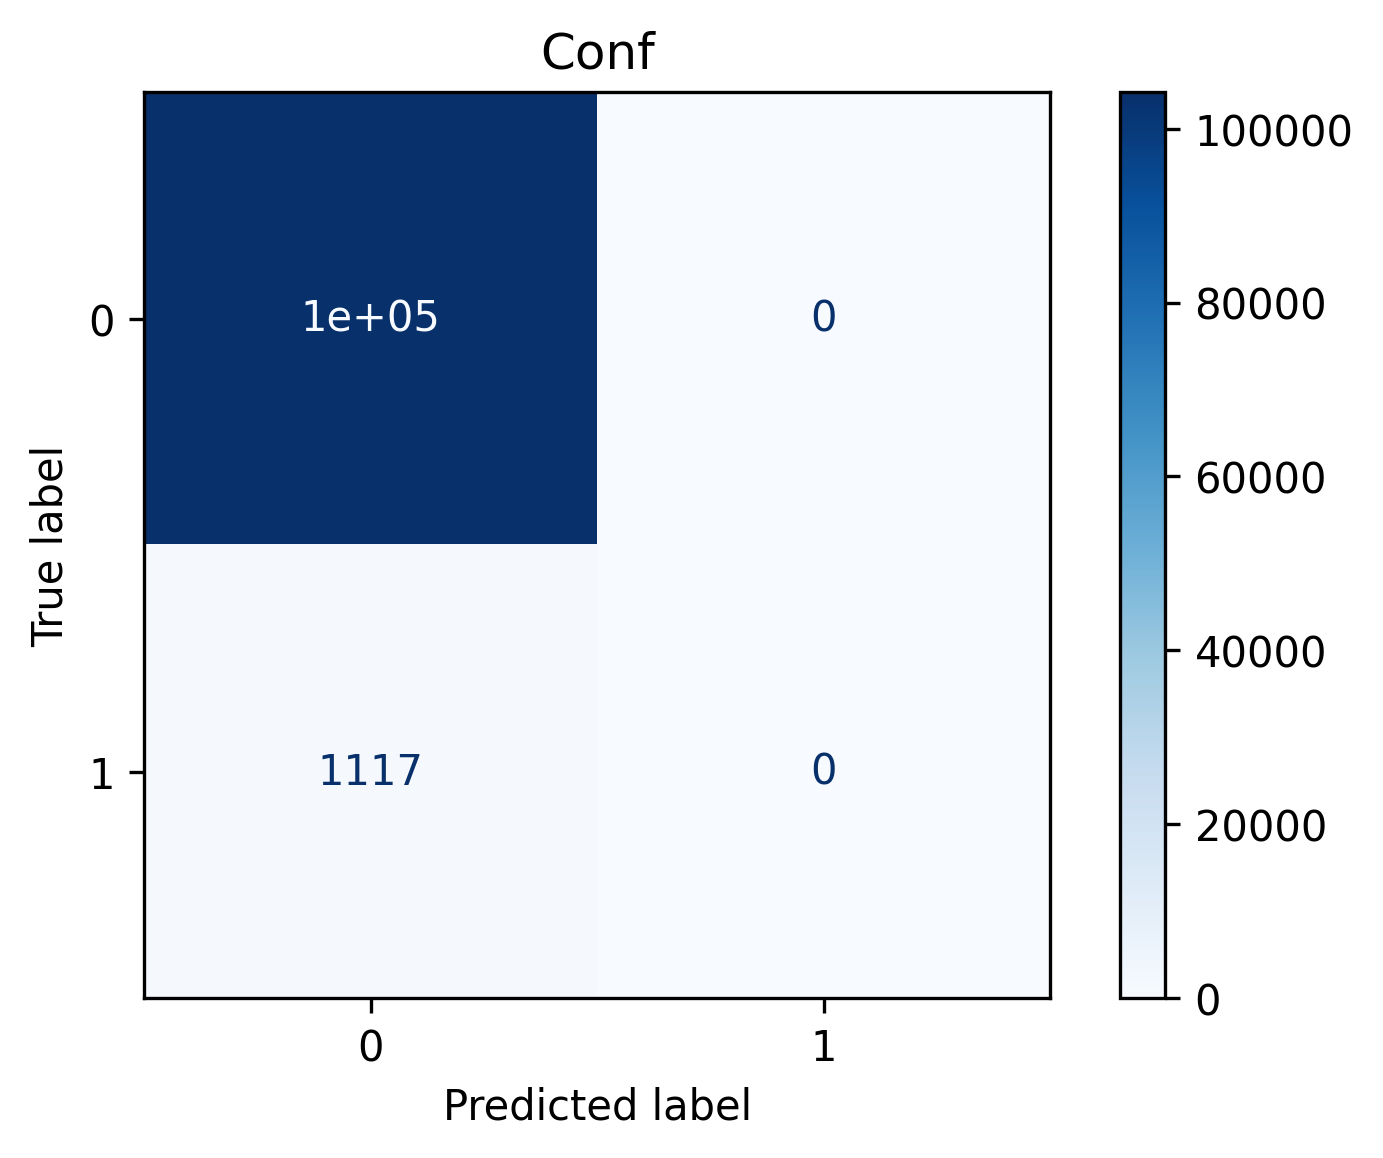
\includegraphics[width=\textwidth]{../images/BiLSTM_train_conf.png}
    \caption{BiLSTM on train}
    \label{fig:BiLSTM_confusion_train}
  \end{subfigure}
  \begin{subfigure}[b]{0.32\textwidth}
    \centering
    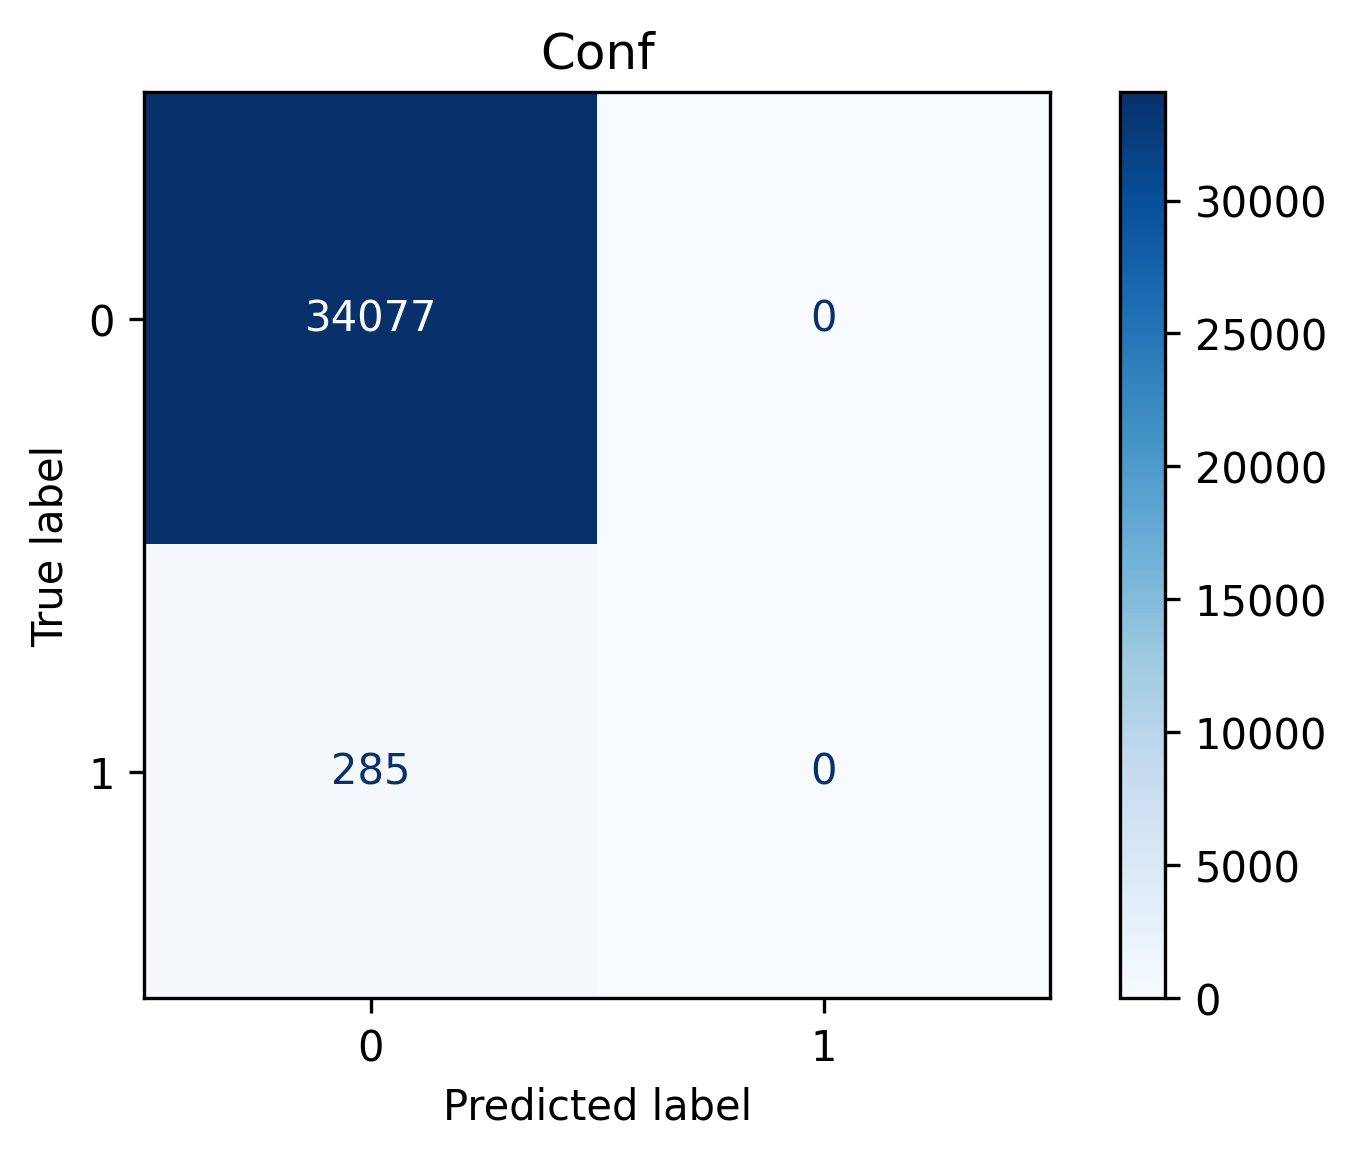
\includegraphics[width=\textwidth]{../images/BiLSTM_val_conf.png}
    \caption{BiLSTM on validation}
    \label{fig:BiLSTM_confusion_val}
  \end{subfigure}
  \begin{subfigure}[b]{0.32\textwidth}
    \centering
    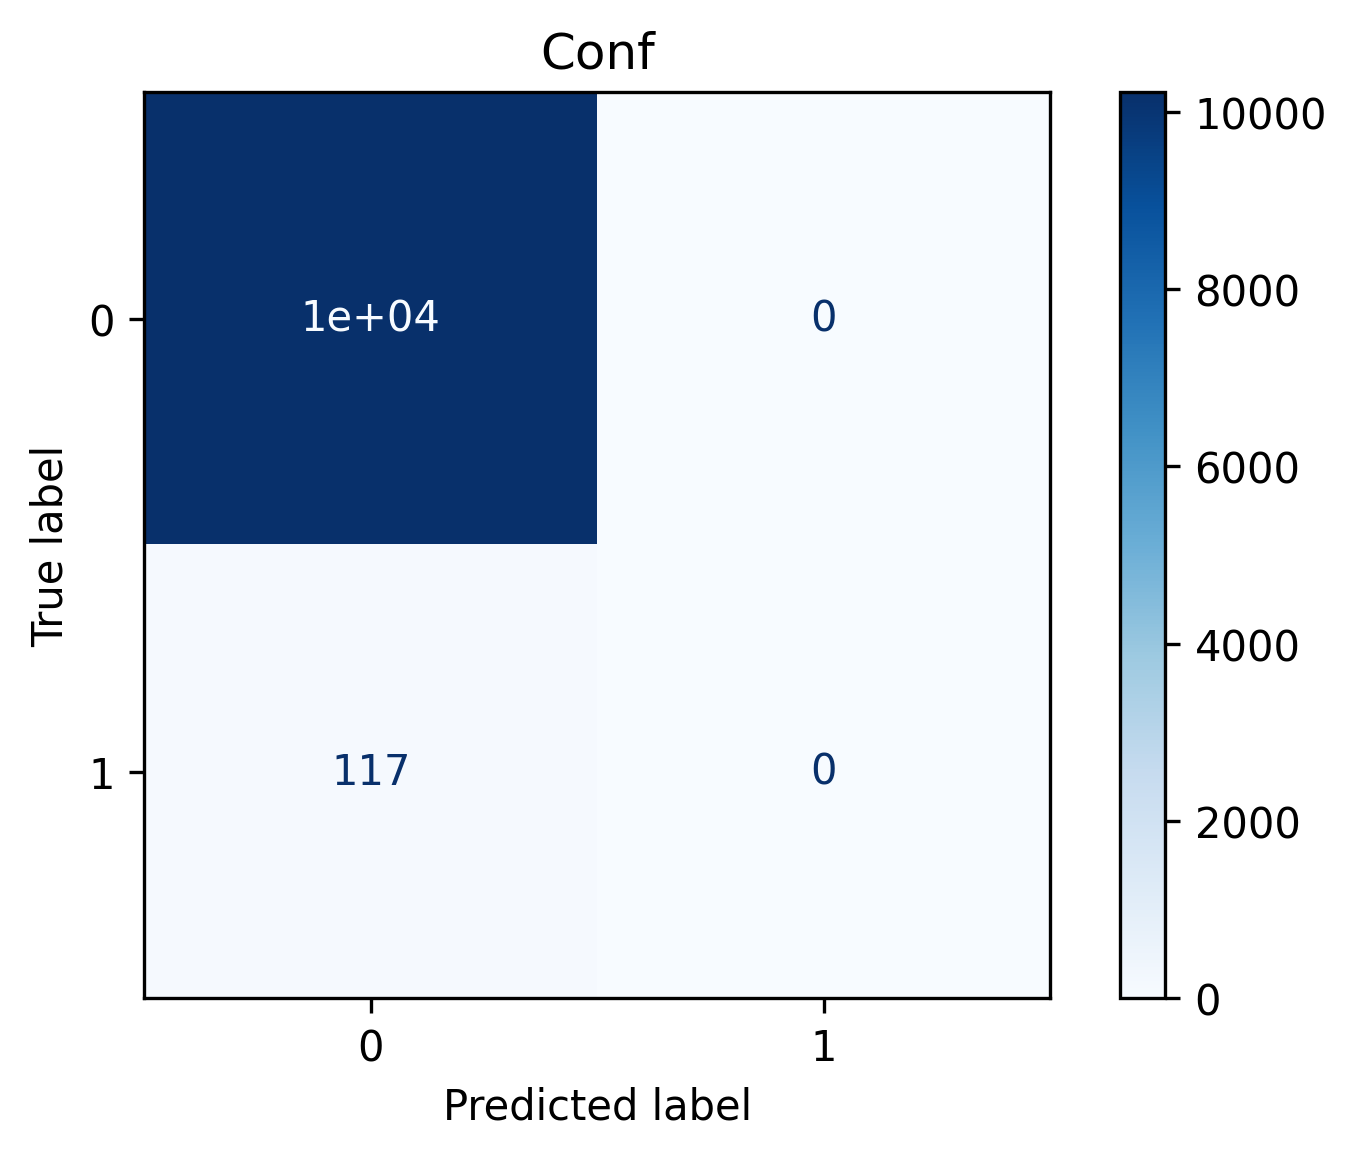
\includegraphics[width=\textwidth]{../images/BiLSTM_test_conf.png}
    \caption{BiLSTM on test}
    \label{fig:BiLSTM_confusion_test}
  \end{subfigure}


  \begin{subfigure}[b]{0.32\textwidth}
    \centering
    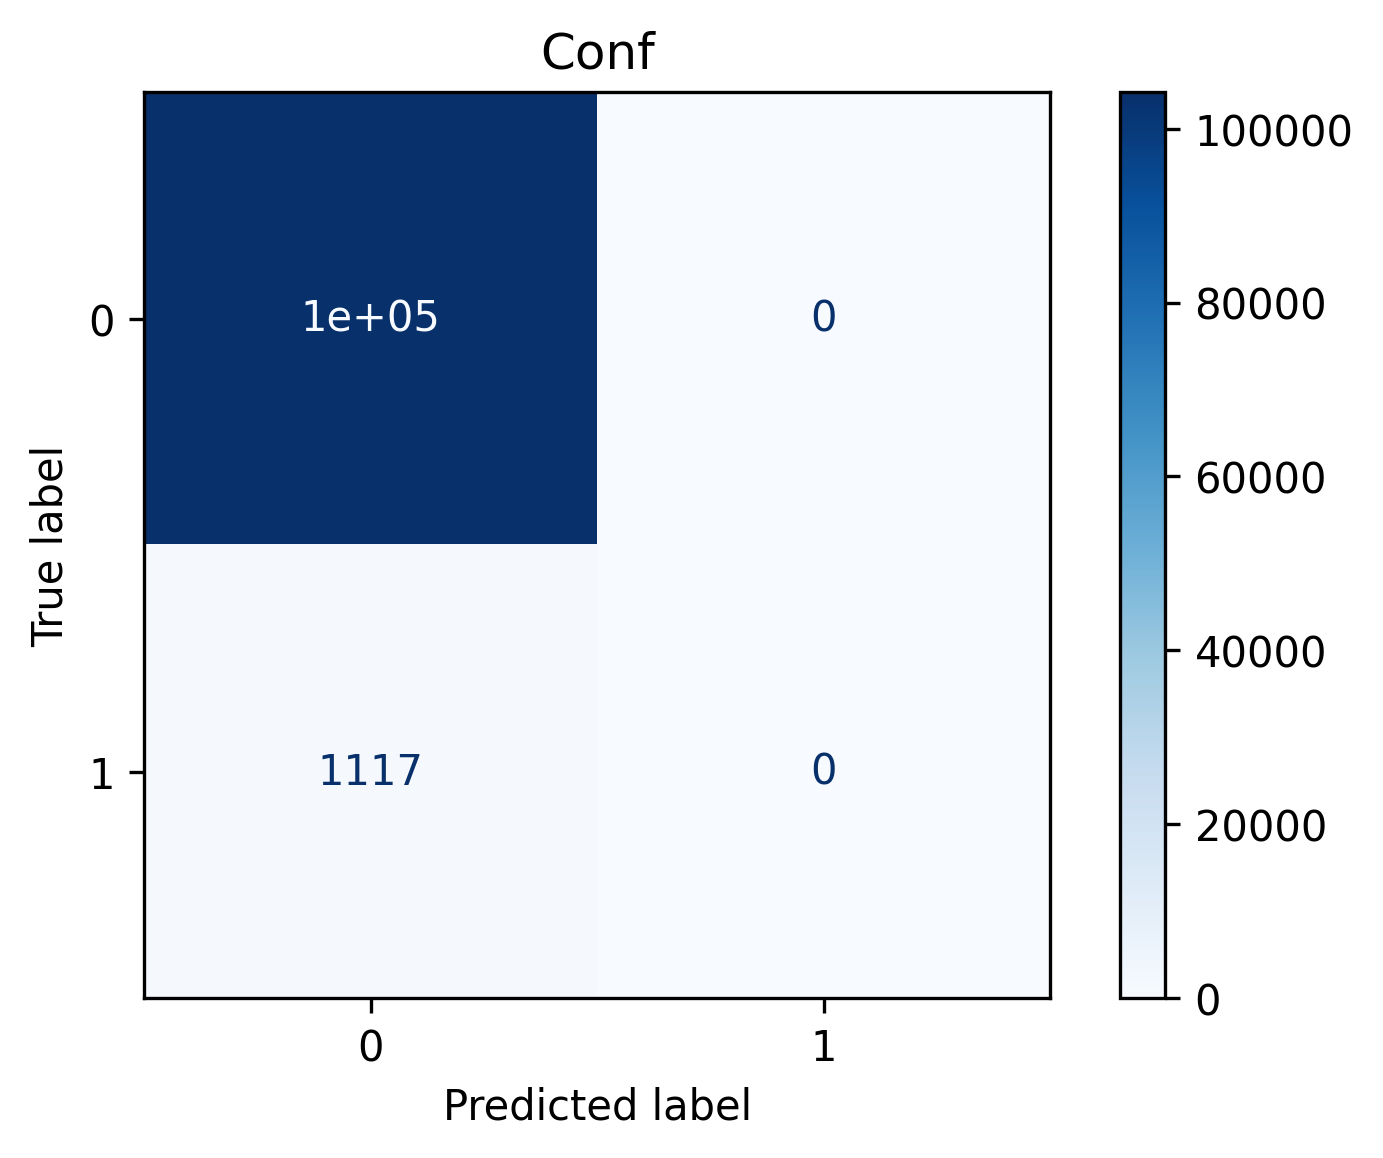
\includegraphics[width=\textwidth]{../images/BiGRU_train_conf.png}
    \caption{BiGRU on train}
    \label{fig:BiGRU_confusion_train}
  \end{subfigure}
  \begin{subfigure}[b]{0.32\textwidth}
    \centering
    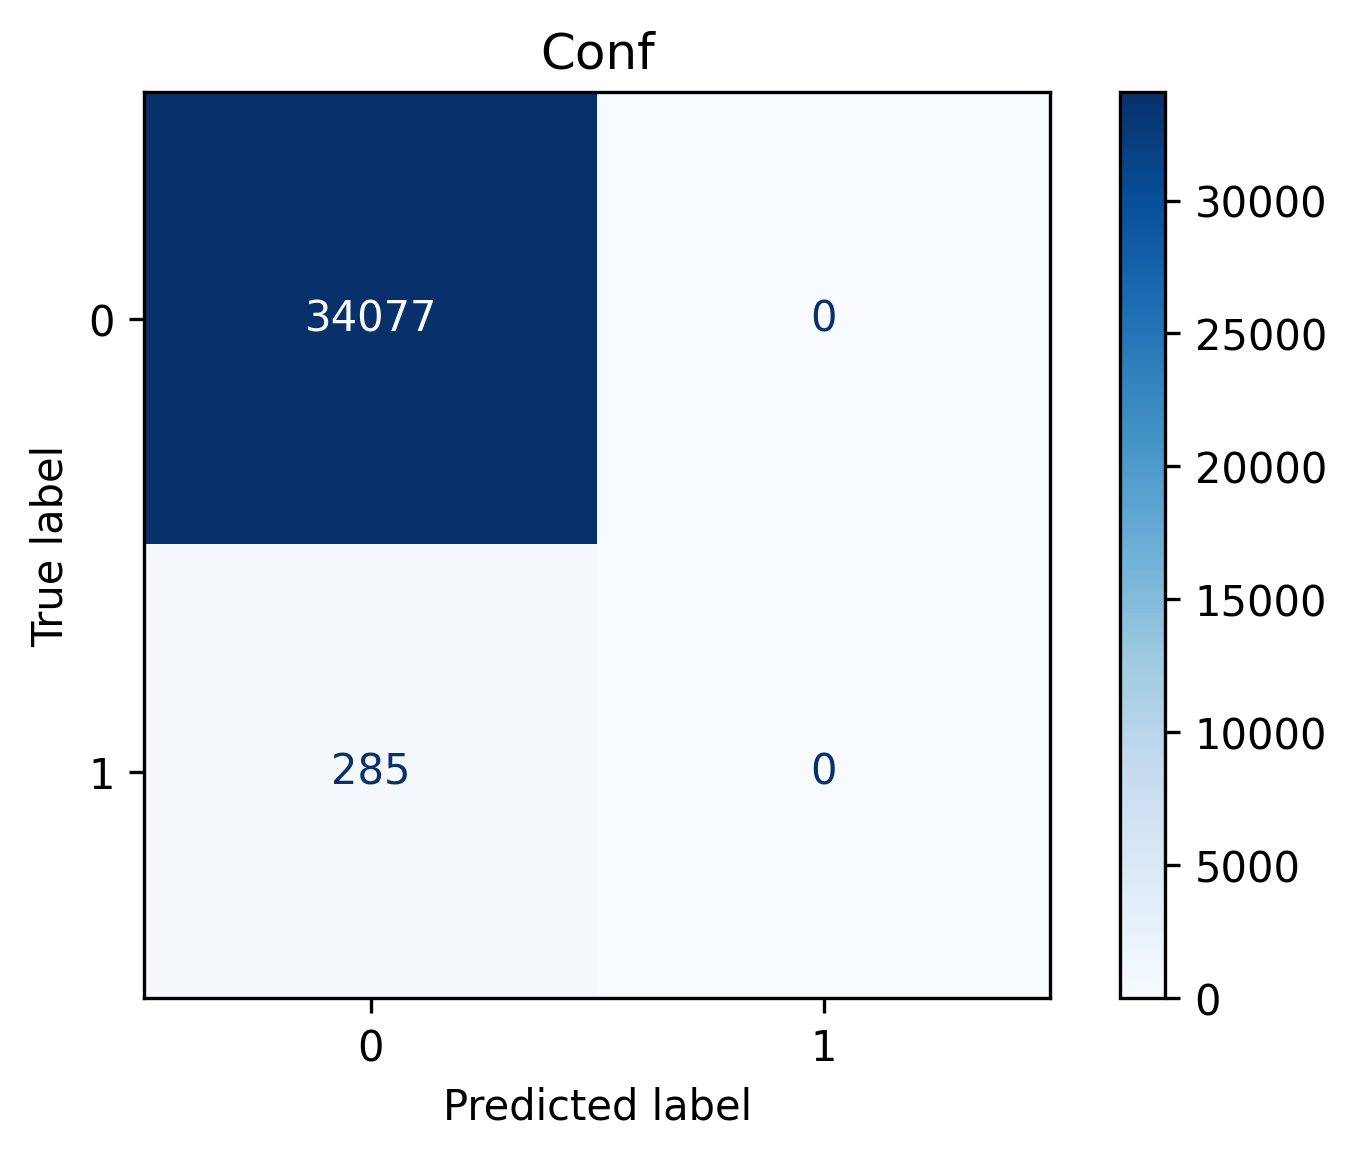
\includegraphics[width=\textwidth]{../images/BiGRU_val_conf.png}
    \caption{BiGRU on validation}
    \label{fig:BiGRU_confusion_val}
  \end{subfigure}
  \begin{subfigure}[b]{0.32\textwidth}
    \centering
    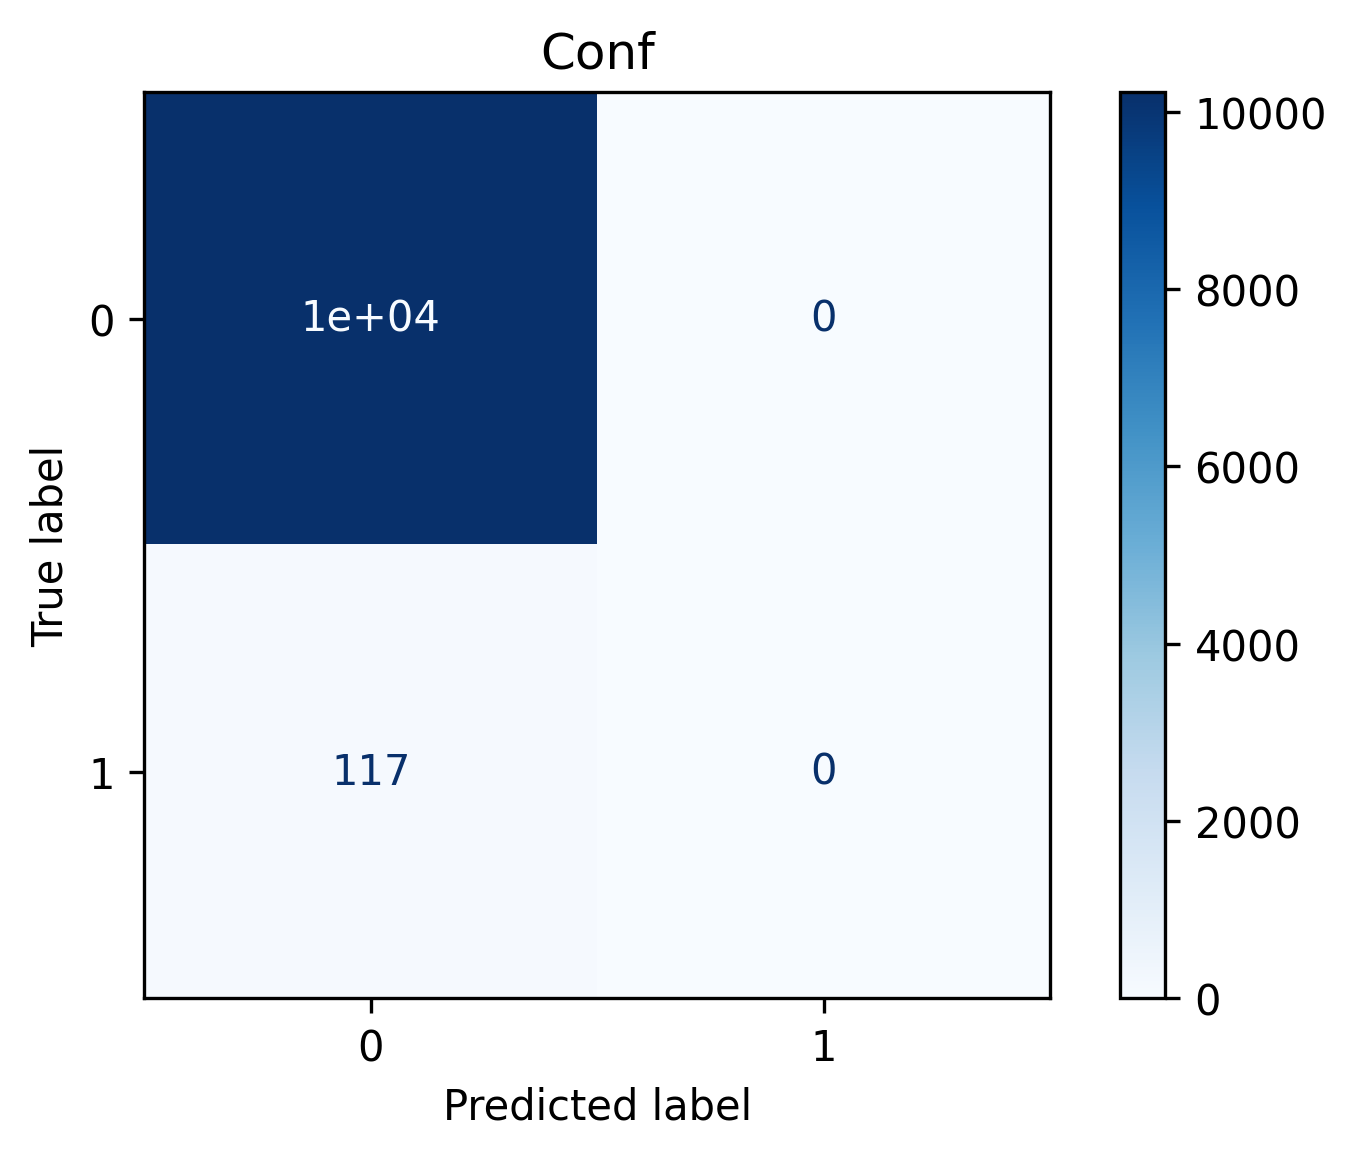
\includegraphics[width=\textwidth]{../images/BiGRU_test_conf.png}
    \caption{BiGRU on test}
    \label{fig:BiGRU_confusion_test}
  \end{subfigure}


  \begin{subfigure}[b]{0.32\textwidth}
    \centering
    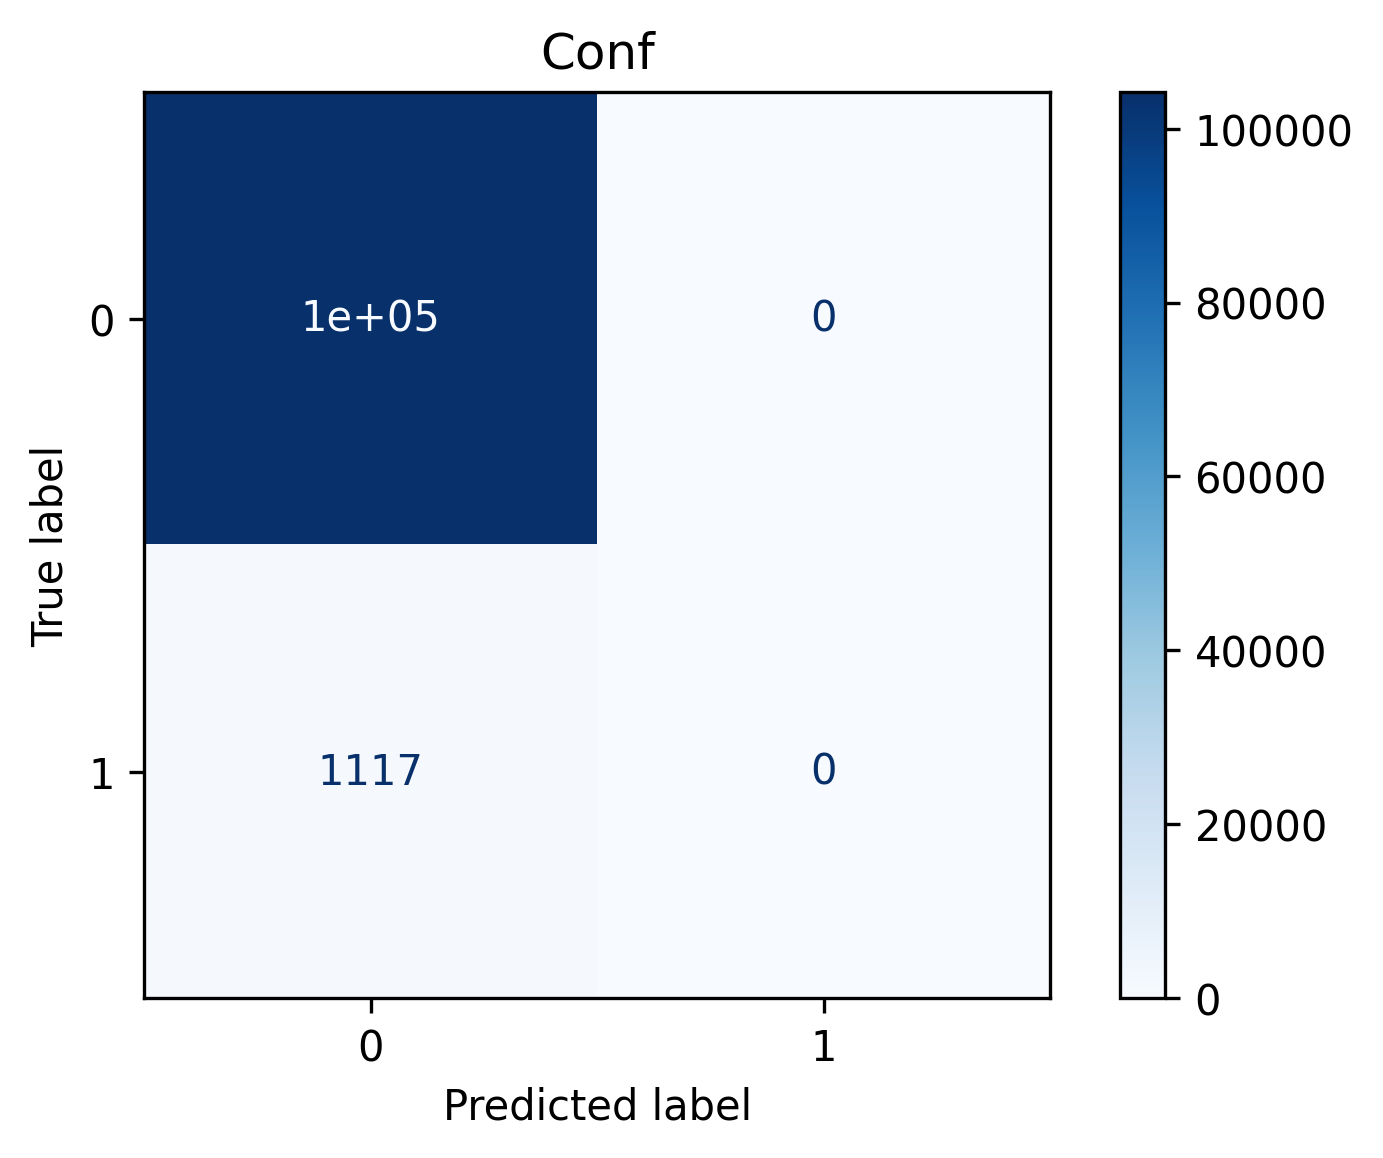
\includegraphics[width=\textwidth]{../images/Transformer_train_conf.png}
    \caption{TEL on train}
    \label{fig:Transformer_confusion_train}
  \end{subfigure}
  \begin{subfigure}[b]{0.32\textwidth}
    \centering
    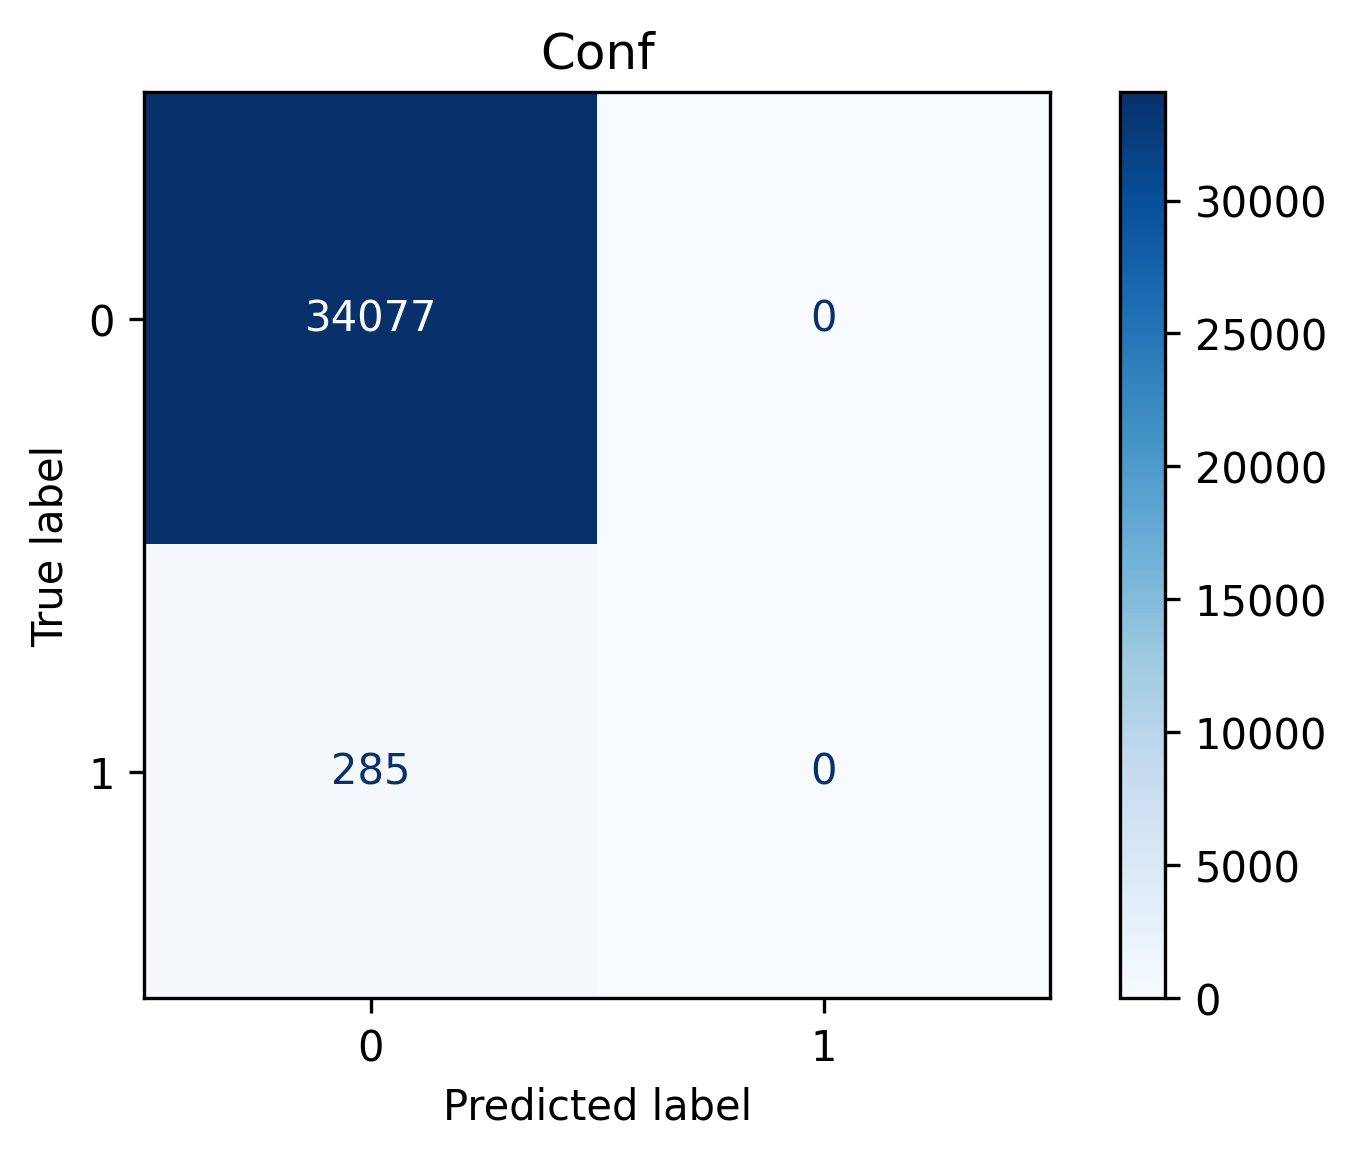
\includegraphics[width=\textwidth]{../images/Transformer_val_conf.png}
    \caption{TEL on validation}
    \label{fig:Transformer_confusion_val}
  \end{subfigure}
  \begin{subfigure}[b]{0.32\textwidth}
    \centering
    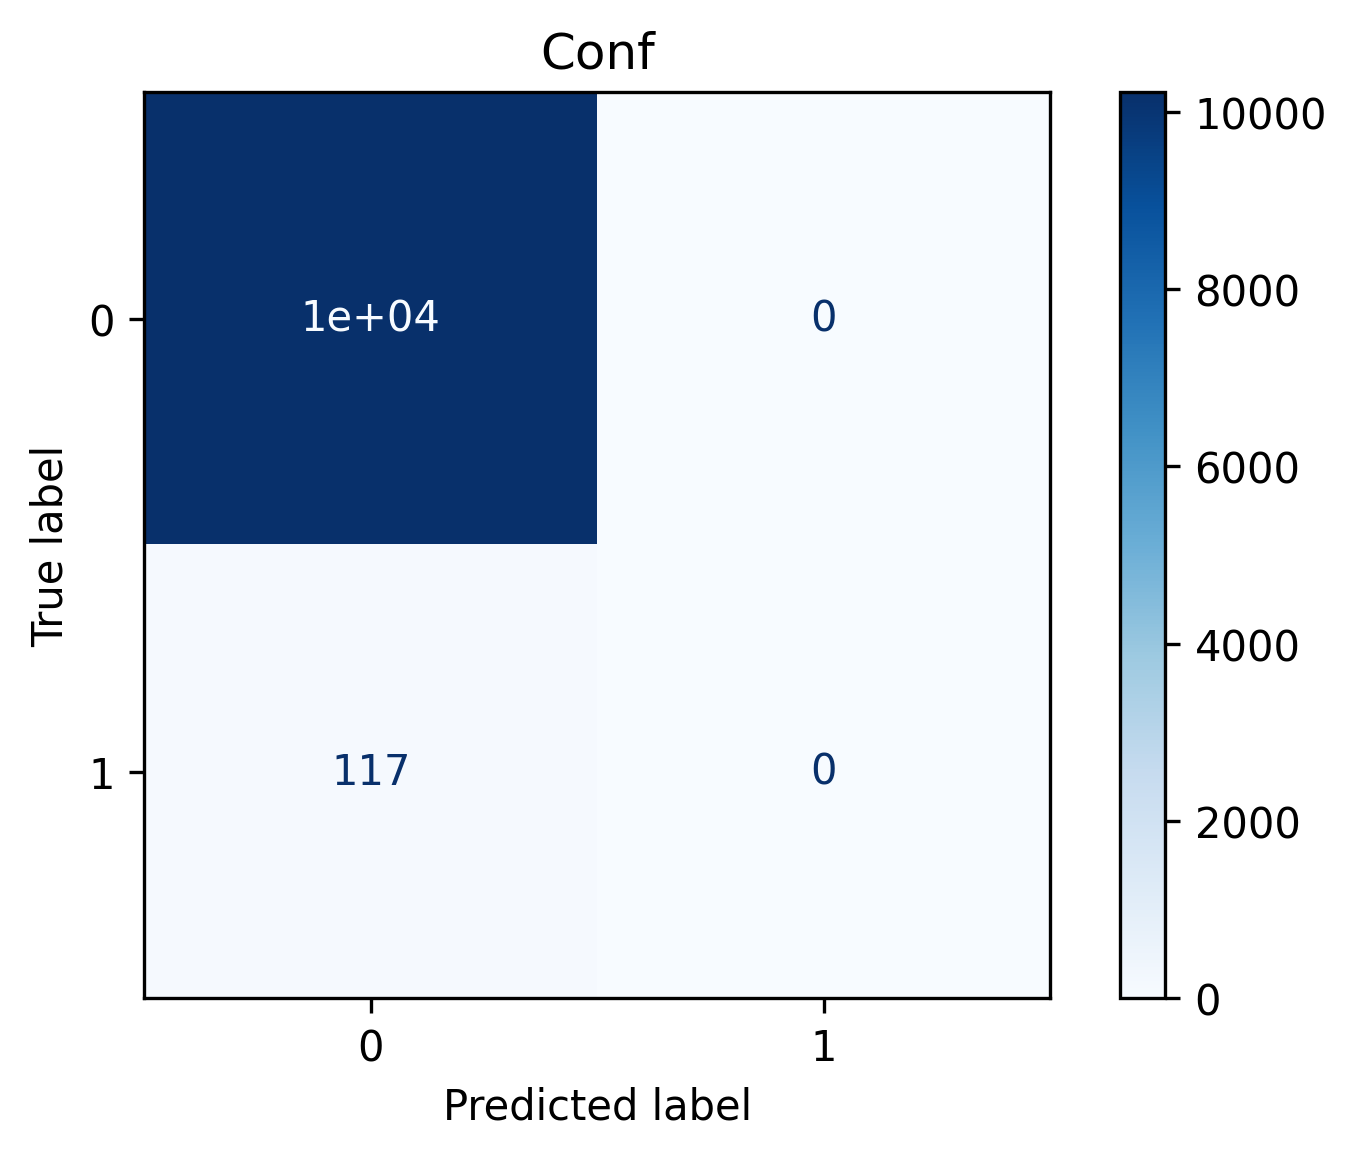
\includegraphics[width=\textwidth]{../images/Transformer_test_conf.png}
    \caption{TEL on test}
    \label{fig:Transformer_confusion_test}
  \end{subfigure}

  \caption{Confusion Matrices}
  \label{fig:confusion}
\end{figure}

\subsection{ROC and PRC}

The ROC curve plots the true-positive rate against the false-positive rate, while the PRC plots precision against recall. In our case we should choose PRC because our data is very imbalanced. The ROC gives a false sense of quality because so many of the non-clicks receive a low probability. ROC curves and PRC curves are shown in  Figure~\ref{fig:roc} and Figure~\ref{fig:prc} respectively.

\begin{figure}[htb]
  \centering
  \begin{subfigure}[b]{0.32\textwidth}
    \centering
    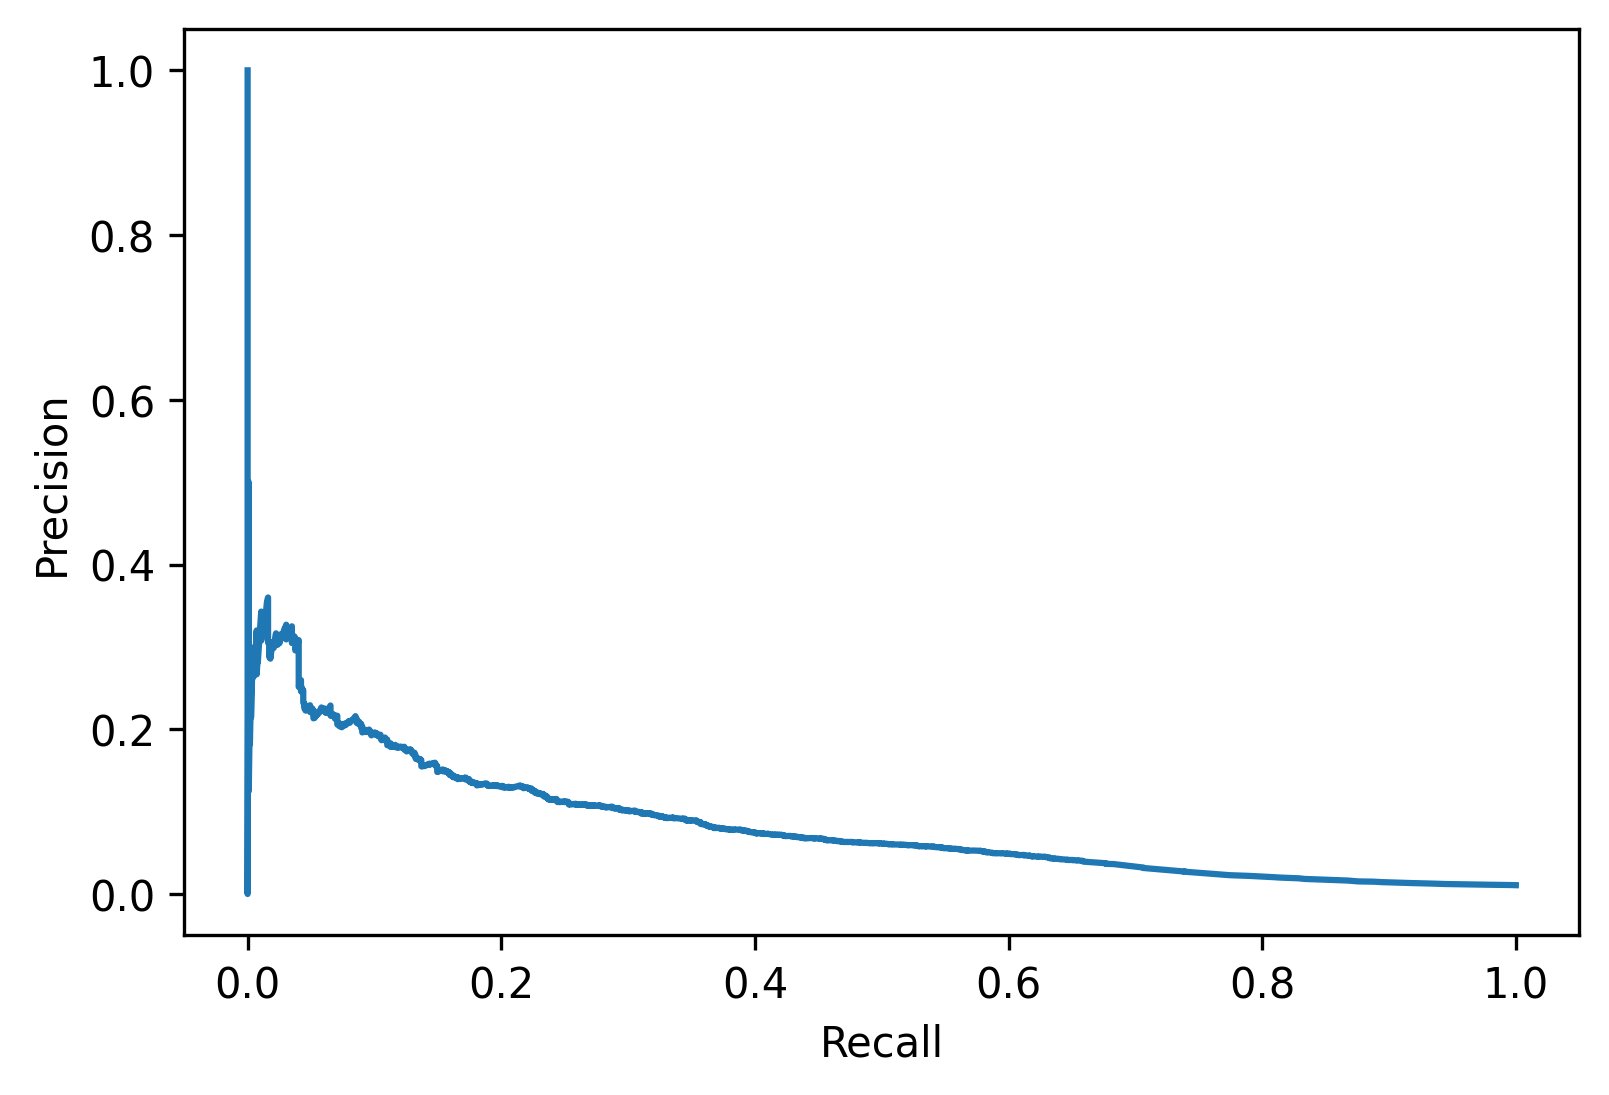
\includegraphics[width=\textwidth]{../images/BiLSTM_train_prc.png}
    \caption{BiLSTM on train}
    \label{fig:BiLSTM_prc_train}
  \end{subfigure}
  \begin{subfigure}[b]{0.32\textwidth}
    \centering
    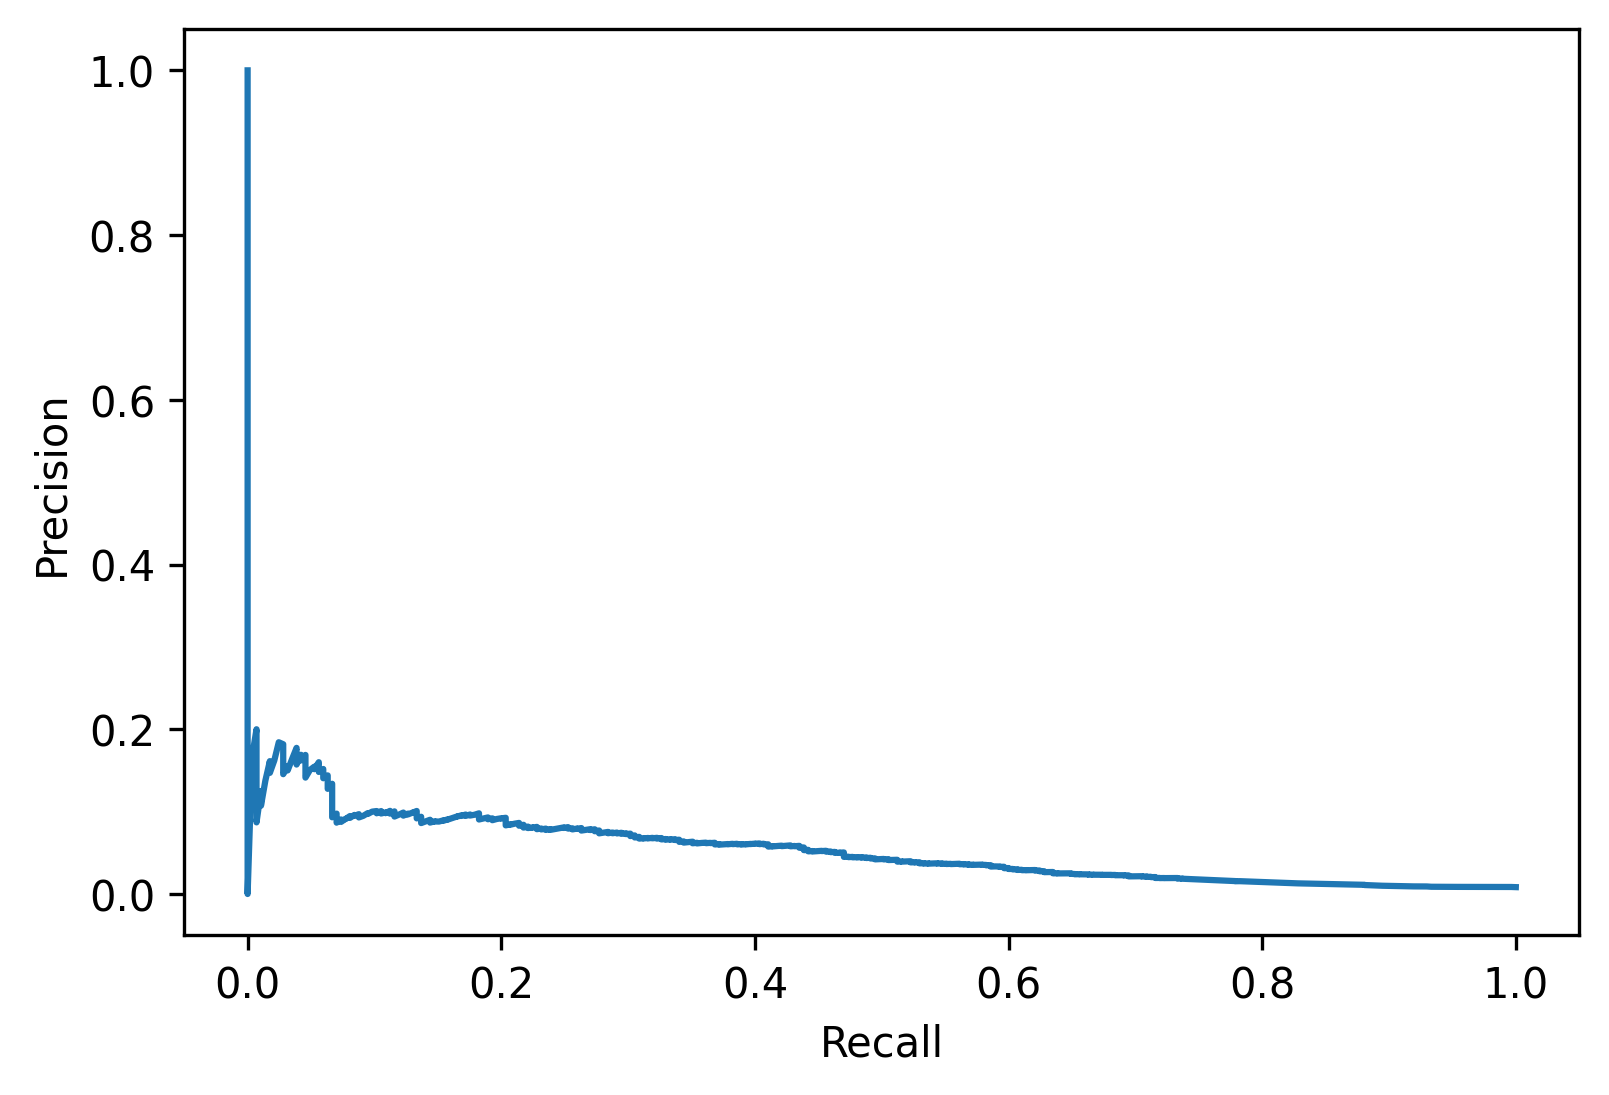
\includegraphics[width=\textwidth]{../images/BiLSTM_val_prc.png}
    \caption{BiLSTM on validation}
    \label{fig:BiLSTM_prc_val}
  \end{subfigure}
  \begin{subfigure}[b]{0.32\textwidth}
    \centering
    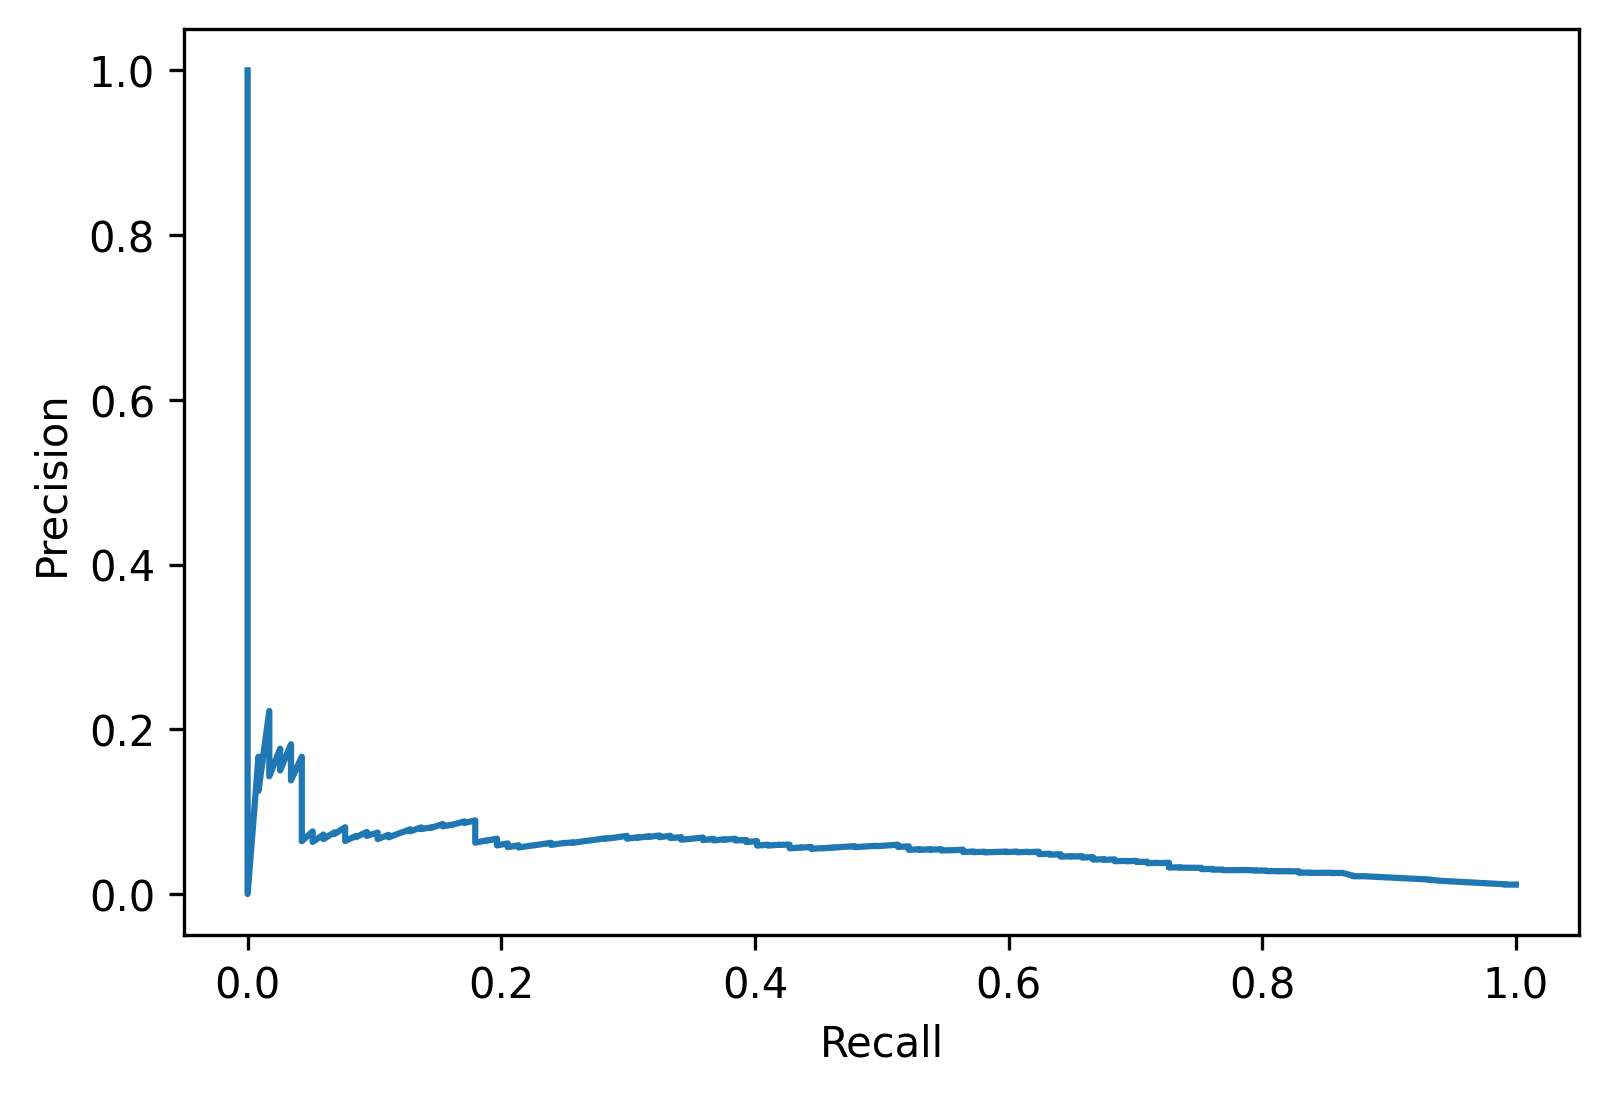
\includegraphics[width=\textwidth]{../images/BiLSTM_test_prc.png}
    \caption{BiLSTM on test}
    \label{fig:BiLSTM_prc_test}
  \end{subfigure}


  \begin{subfigure}[b]{0.32\textwidth}
    \centering
    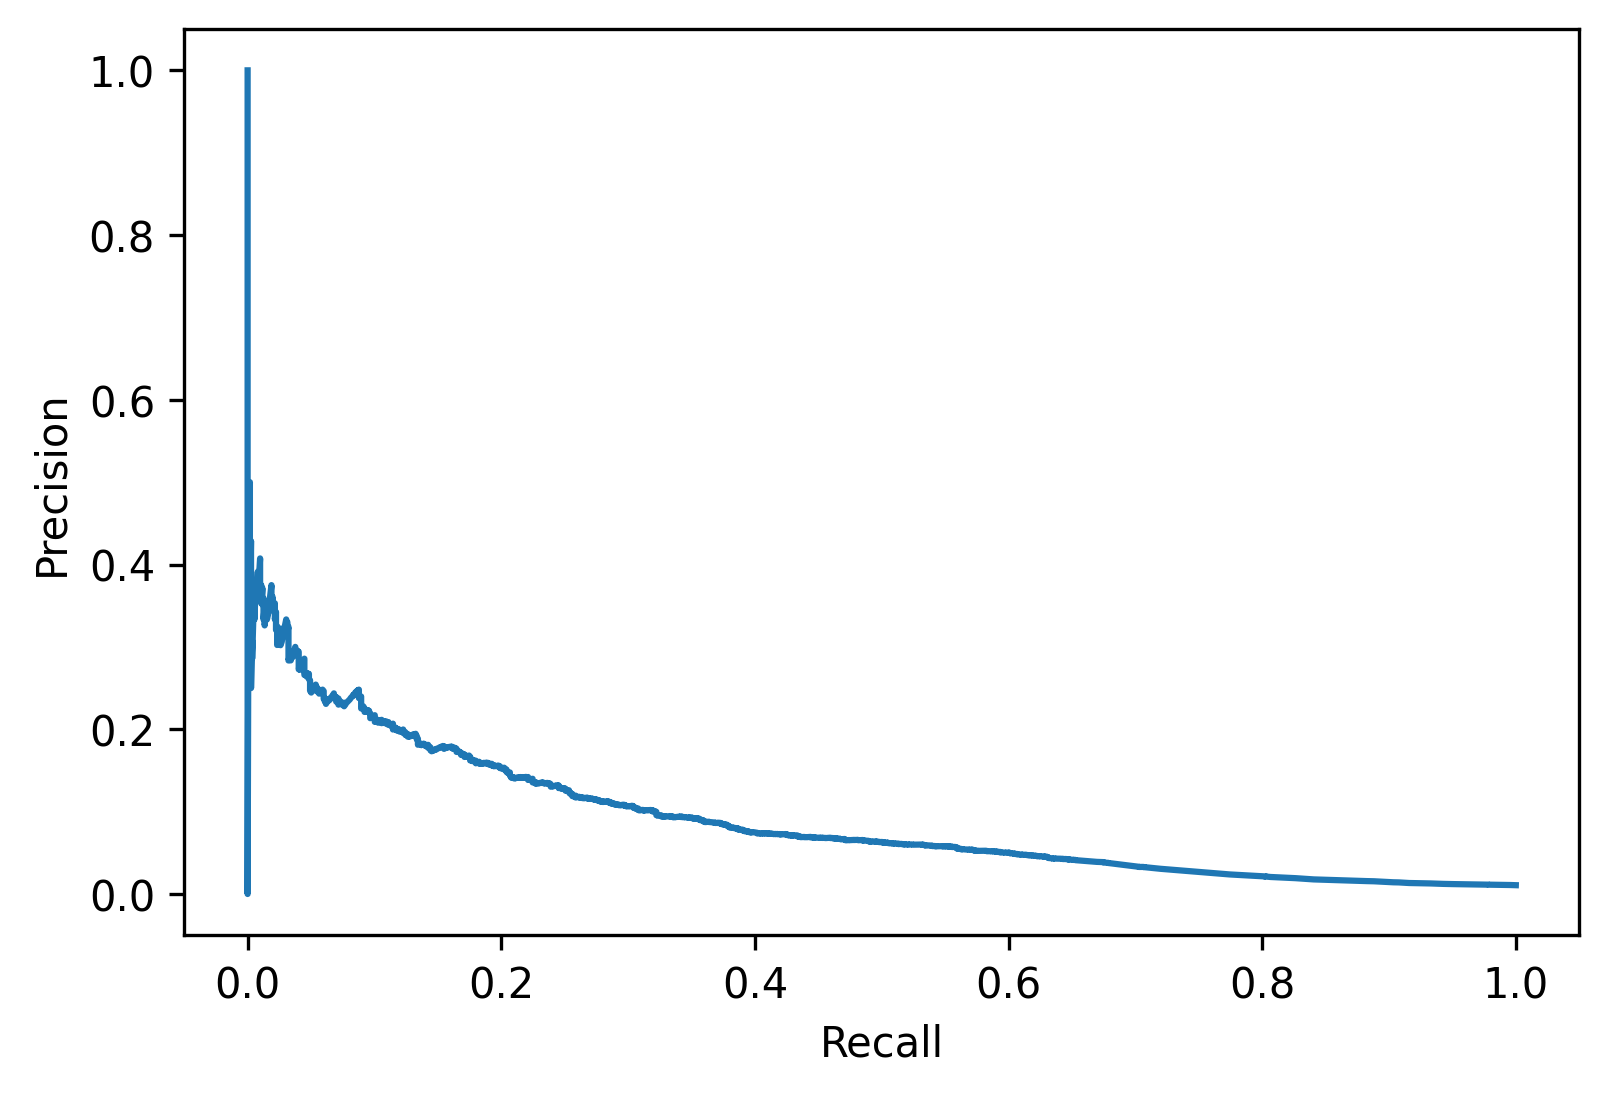
\includegraphics[width=\textwidth]{../images/BiGRU_train_prc.png}
    \caption{BiGRU on train}
    \label{fig:BiGRU_prc_train}
  \end{subfigure}
  \begin{subfigure}[b]{0.32\textwidth}
    \centering
    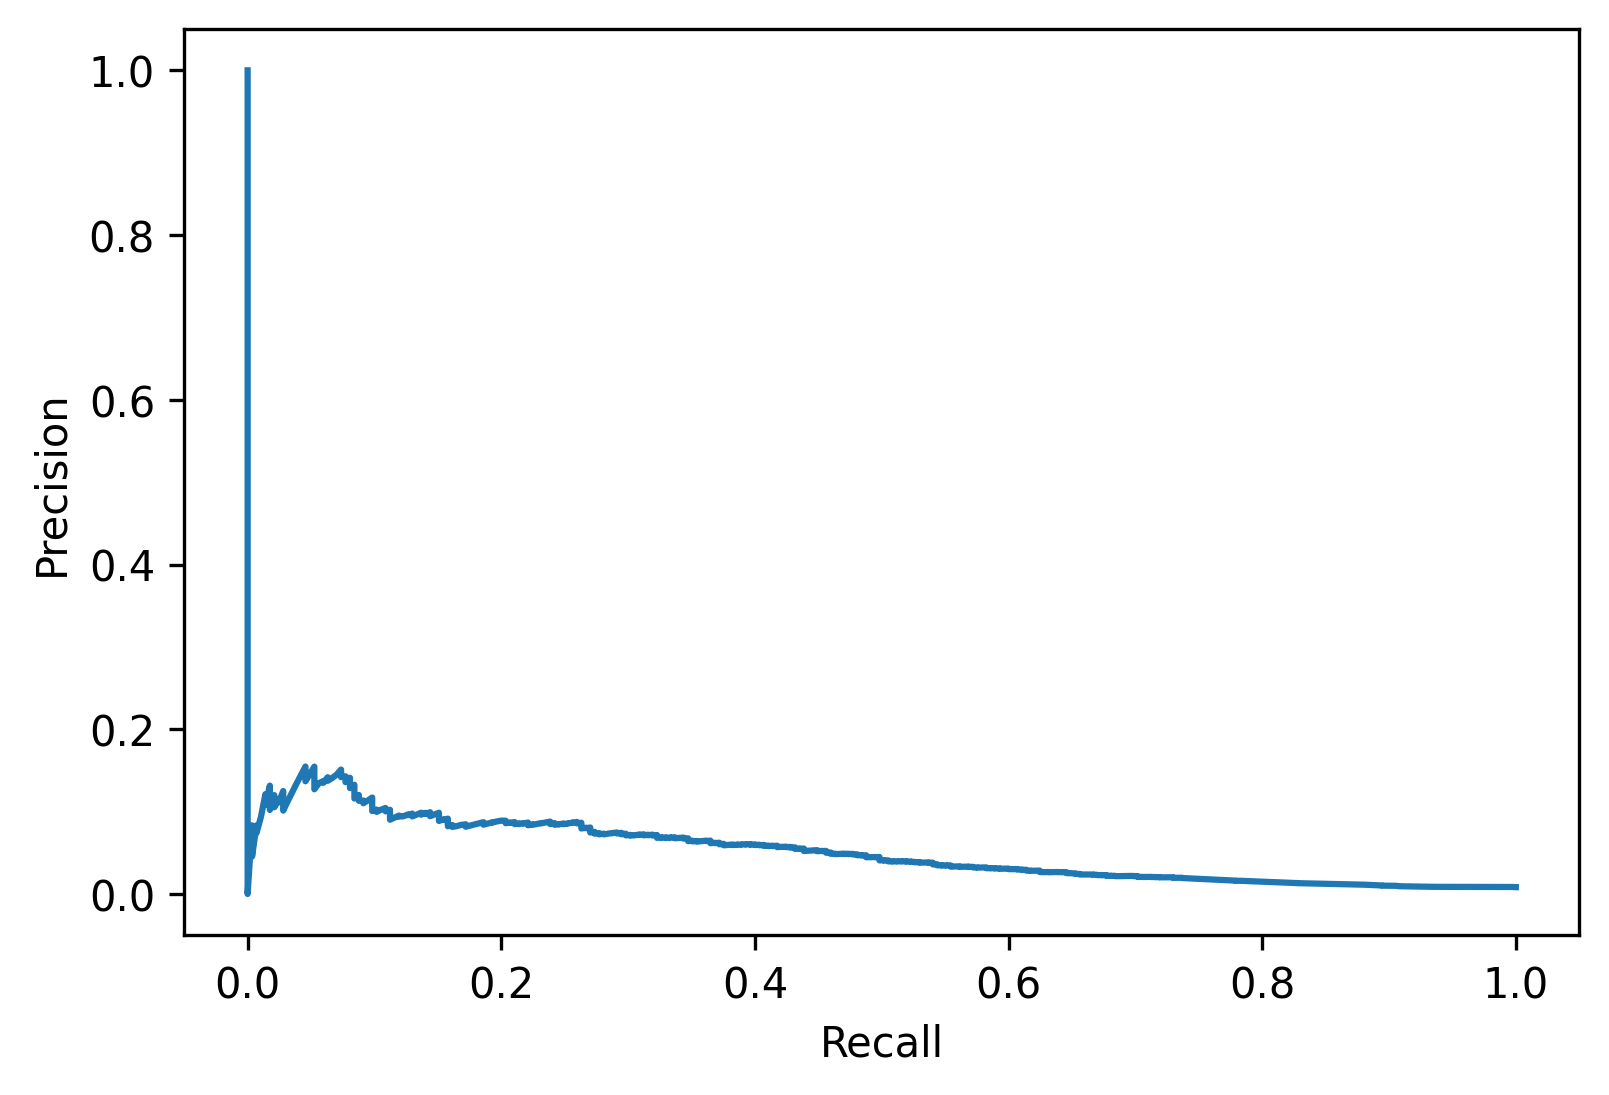
\includegraphics[width=\textwidth]{../images/BiGRU_val_prc.png}
    \caption{BiGRU on validation}
    \label{fig:BiGRU_prc_val}
  \end{subfigure}
  \begin{subfigure}[b]{0.32\textwidth}
    \centering
    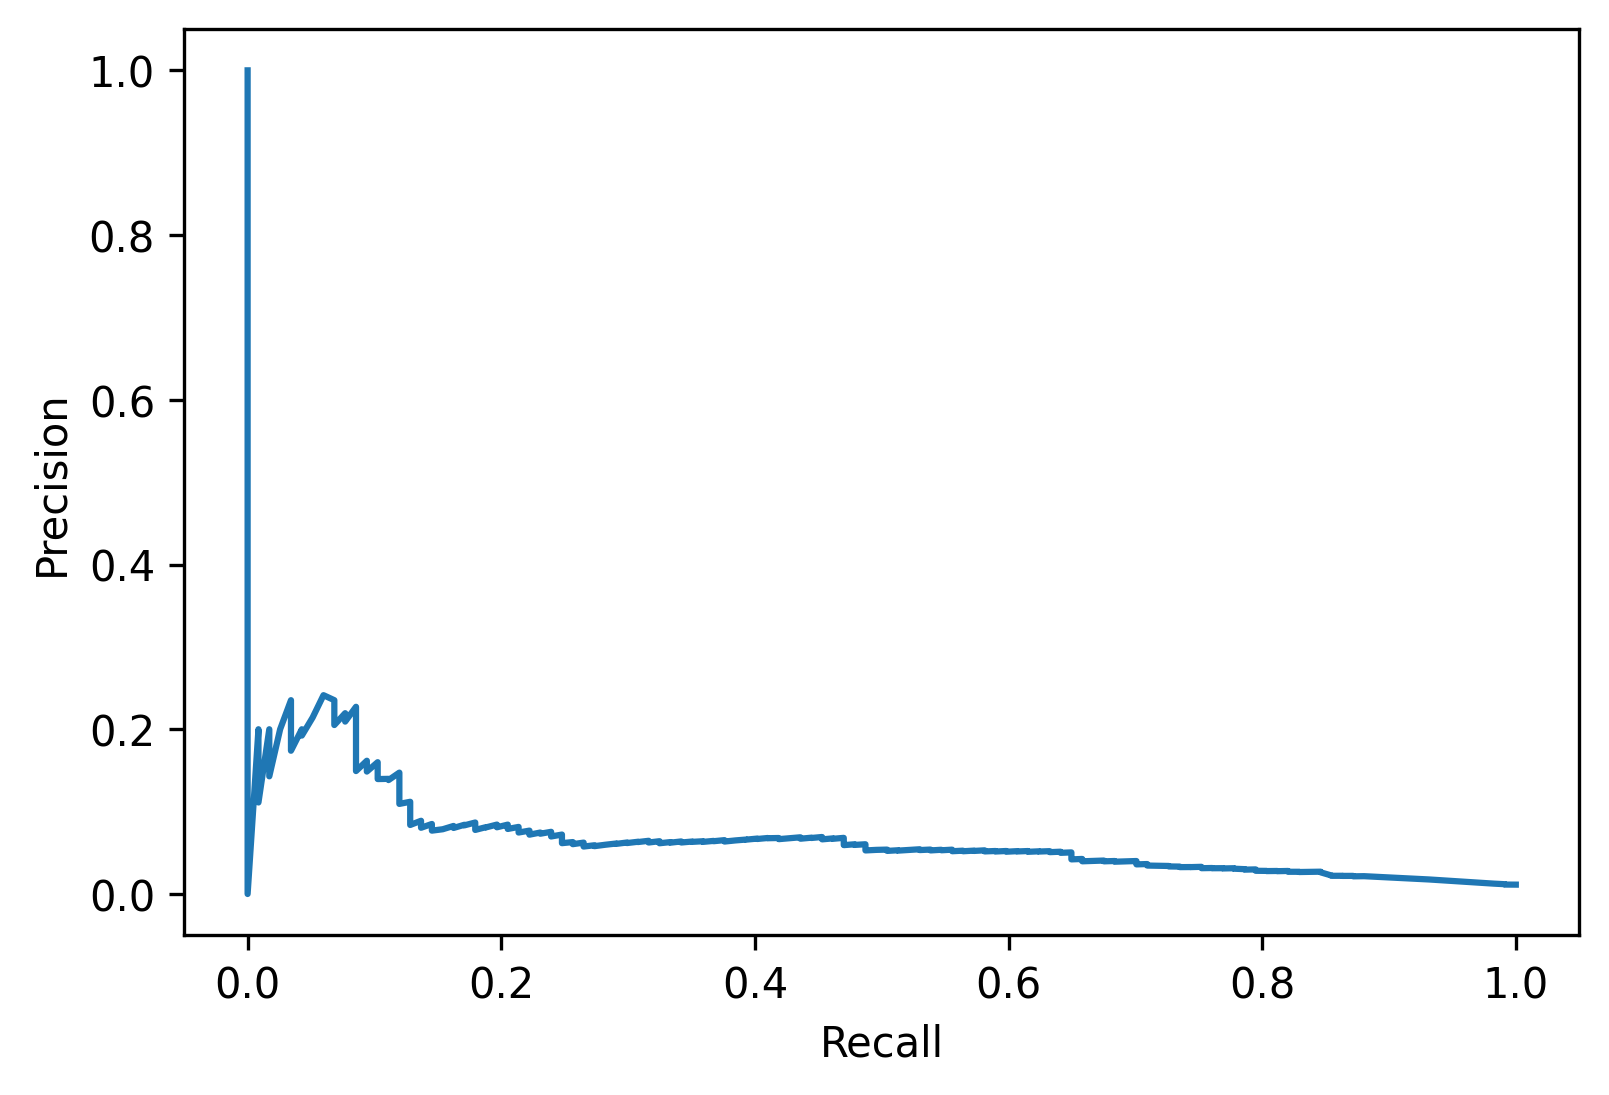
\includegraphics[width=\textwidth]{../images/BiGRU_test_prc.png}
    \caption{BiGRU on test}
    \label{fig:BiGRU_prc_test}
  \end{subfigure}


  \begin{subfigure}[b]{0.32\textwidth}
    \centering
    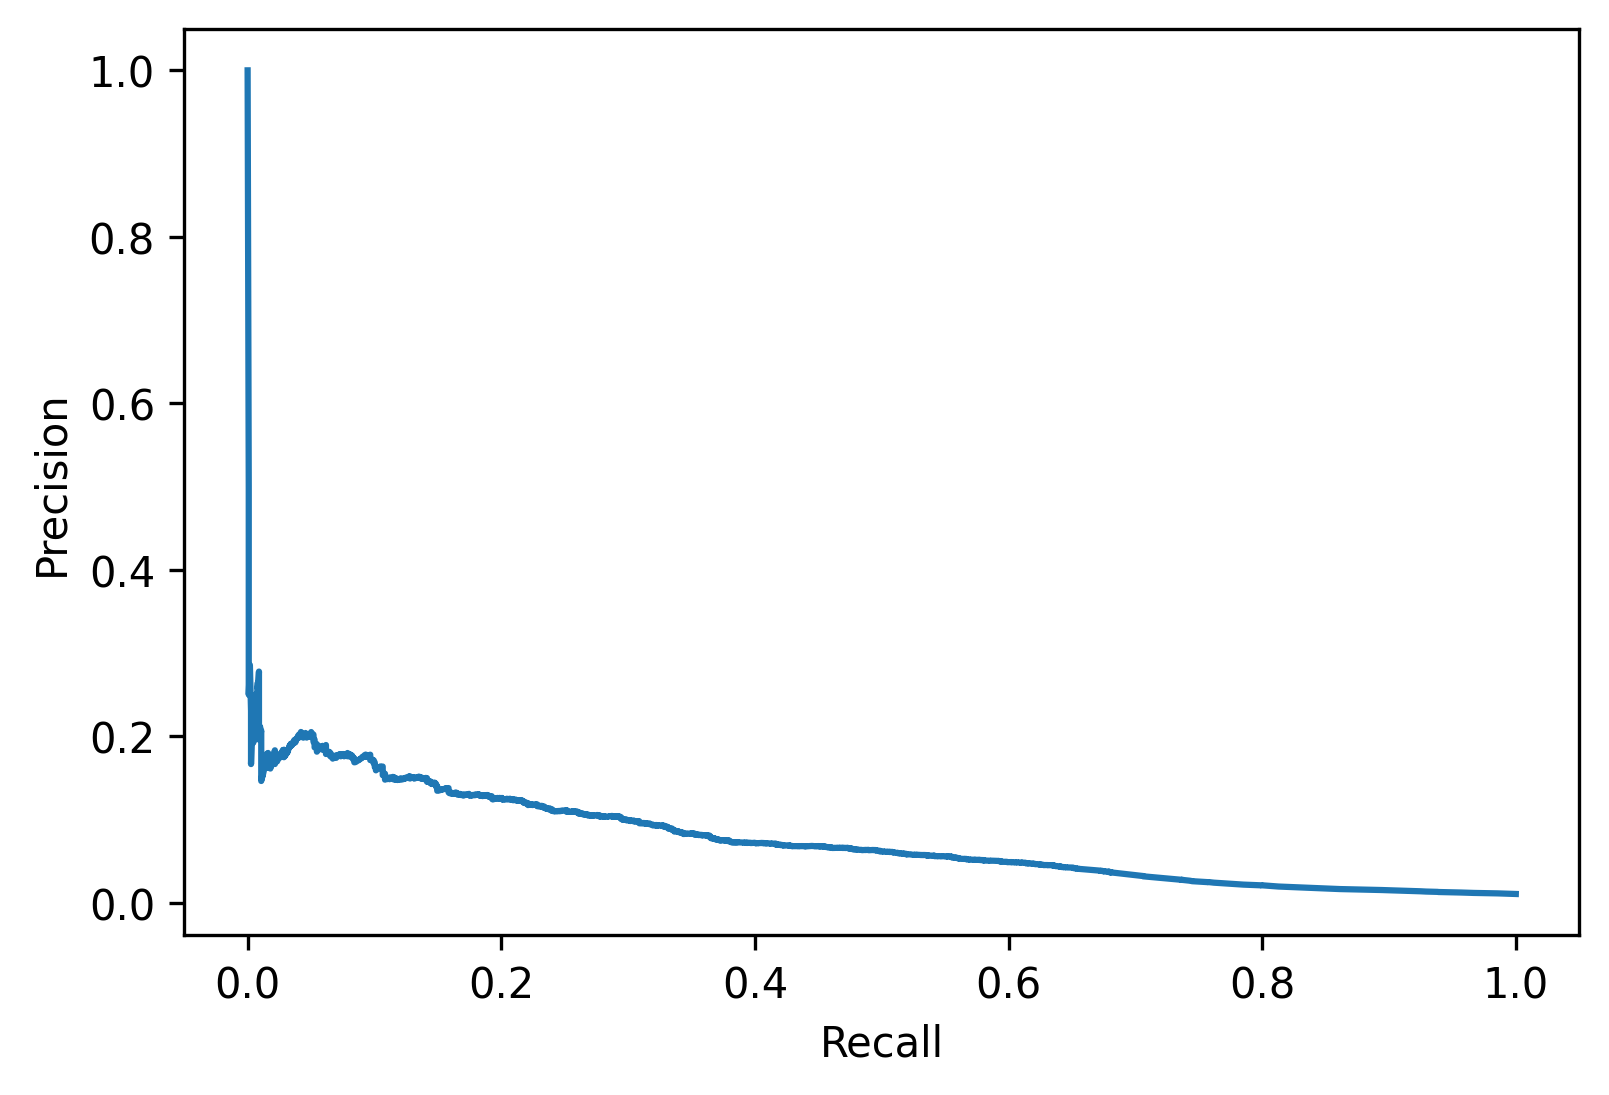
\includegraphics[width=\textwidth]{../images/Transformer_train_prc.png}
    \caption{TEL on train}
    \label{fig:Transformer_prc_train}
  \end{subfigure}
  \begin{subfigure}[b]{0.32\textwidth}
    \centering
    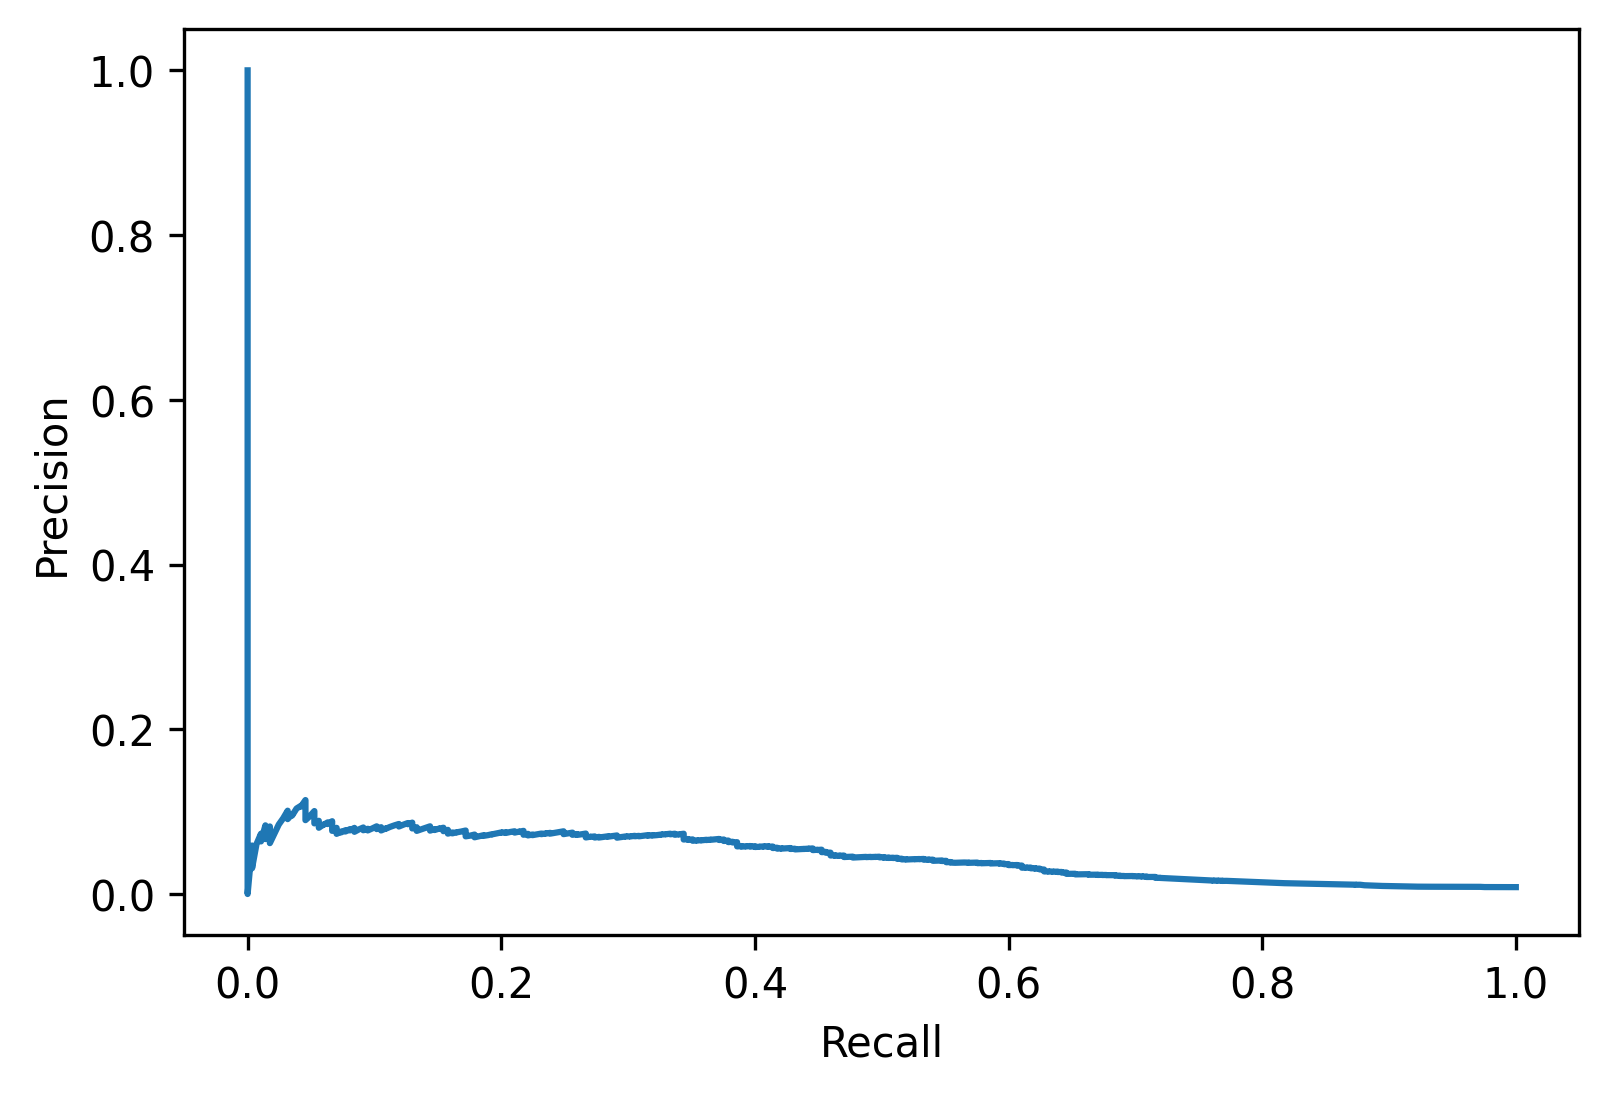
\includegraphics[width=\textwidth]{../images/Transformer_val_prc.png}
    \caption{TEL on validation}
    \label{fig:Transformer_prc_val}
  \end{subfigure}
  \begin{subfigure}[b]{0.32\textwidth}
    \centering
    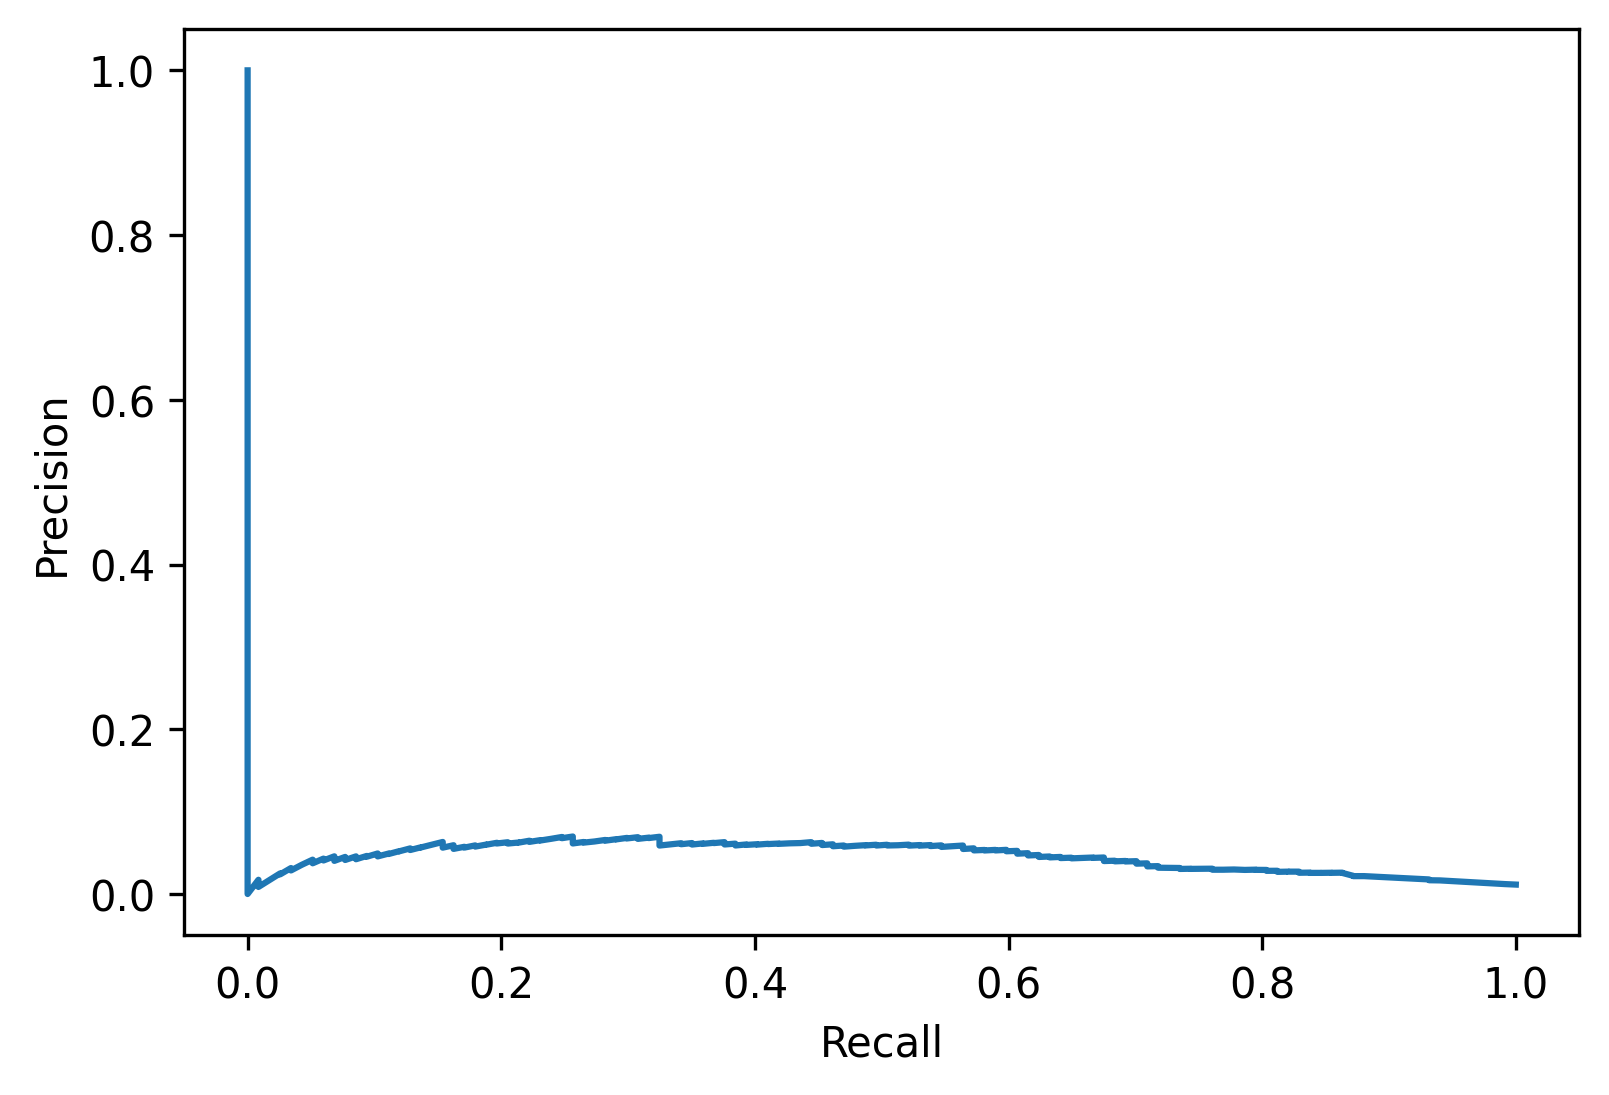
\includegraphics[width=\textwidth]{../images/Transformer_test_prc.png}
    \caption{TEL on test}
    \label{fig:Transformer_prc_test}
  \end{subfigure}

  \caption{Precision recall curves}
  \label{fig:prc}
\end{figure}


\begin{figure}[htb]
  \centering
  \begin{subfigure}[b]{0.32\textwidth}
    \centering
    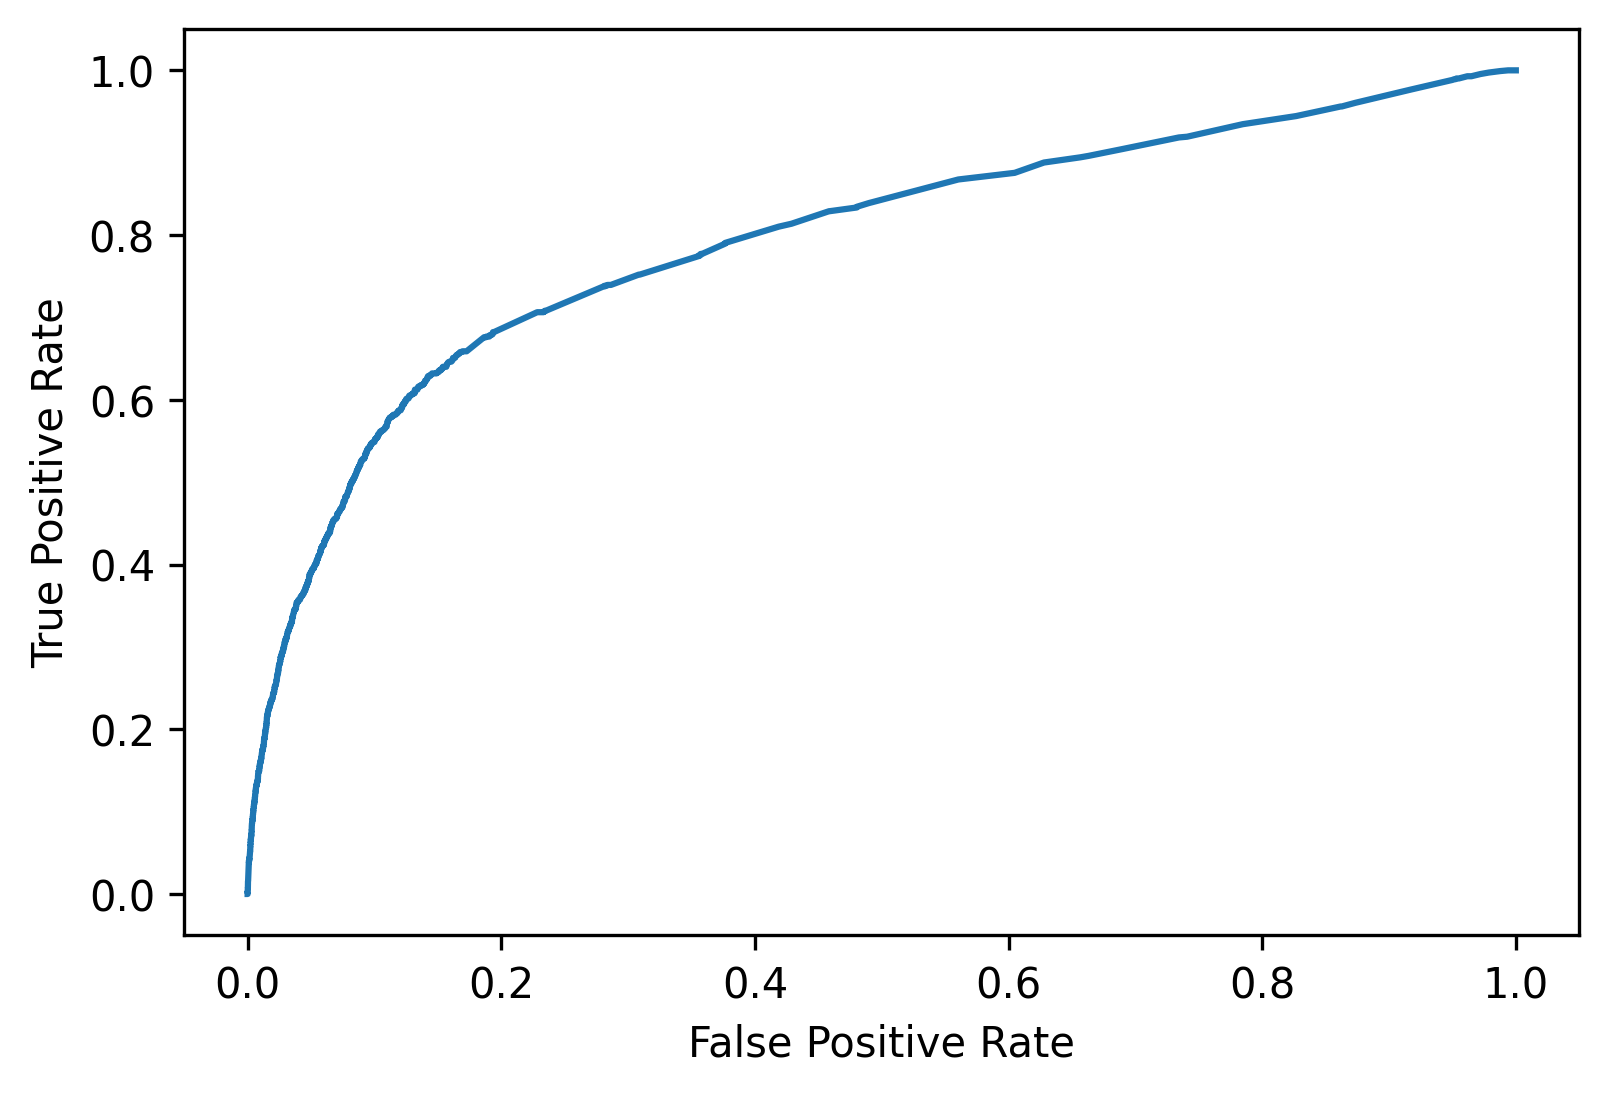
\includegraphics[width=\textwidth]{../images/BiLSTM_train_roc.png}
    \caption{BiLSTM on train}
    \label{fig:BiLSTM_roc_train}
  \end{subfigure}
  \begin{subfigure}[b]{0.32\textwidth}
    \centering
    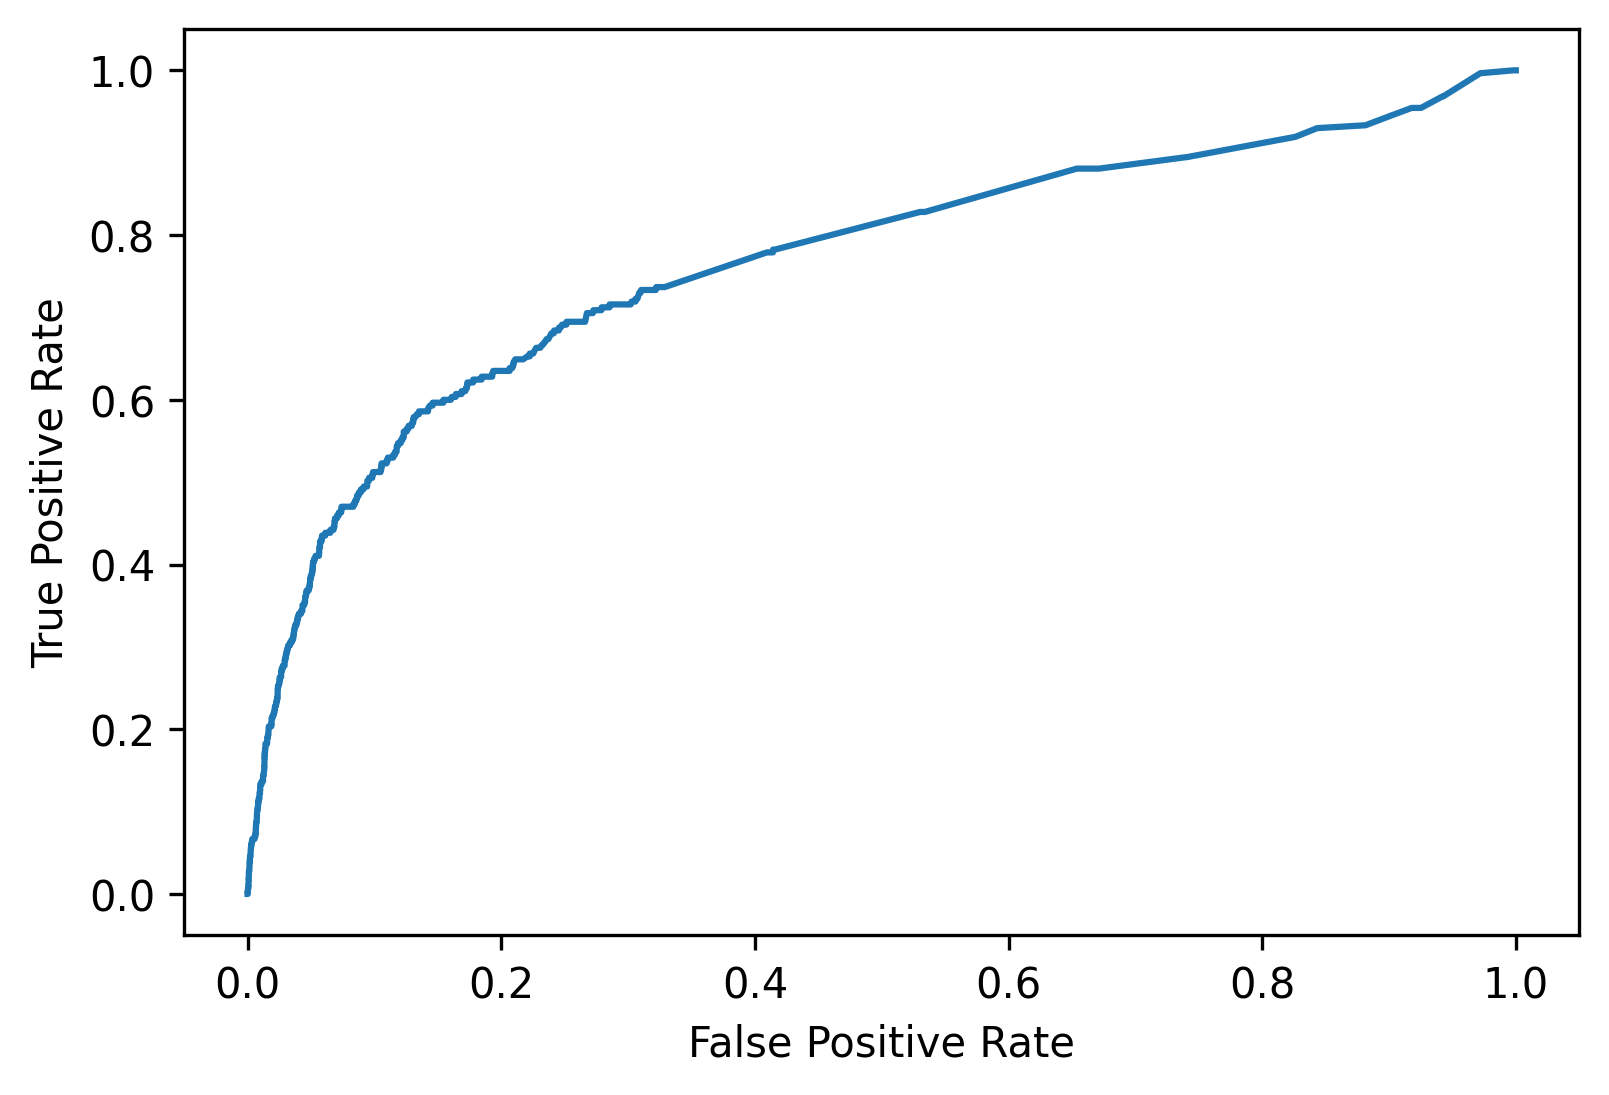
\includegraphics[width=\textwidth]{../images/BiLSTM_val_roc.png}
    \caption{BiLSTM on validation}
    \label{fig:BiLSTM_roc_val}
  \end{subfigure}
  \begin{subfigure}[b]{0.32\textwidth}
    \centering
    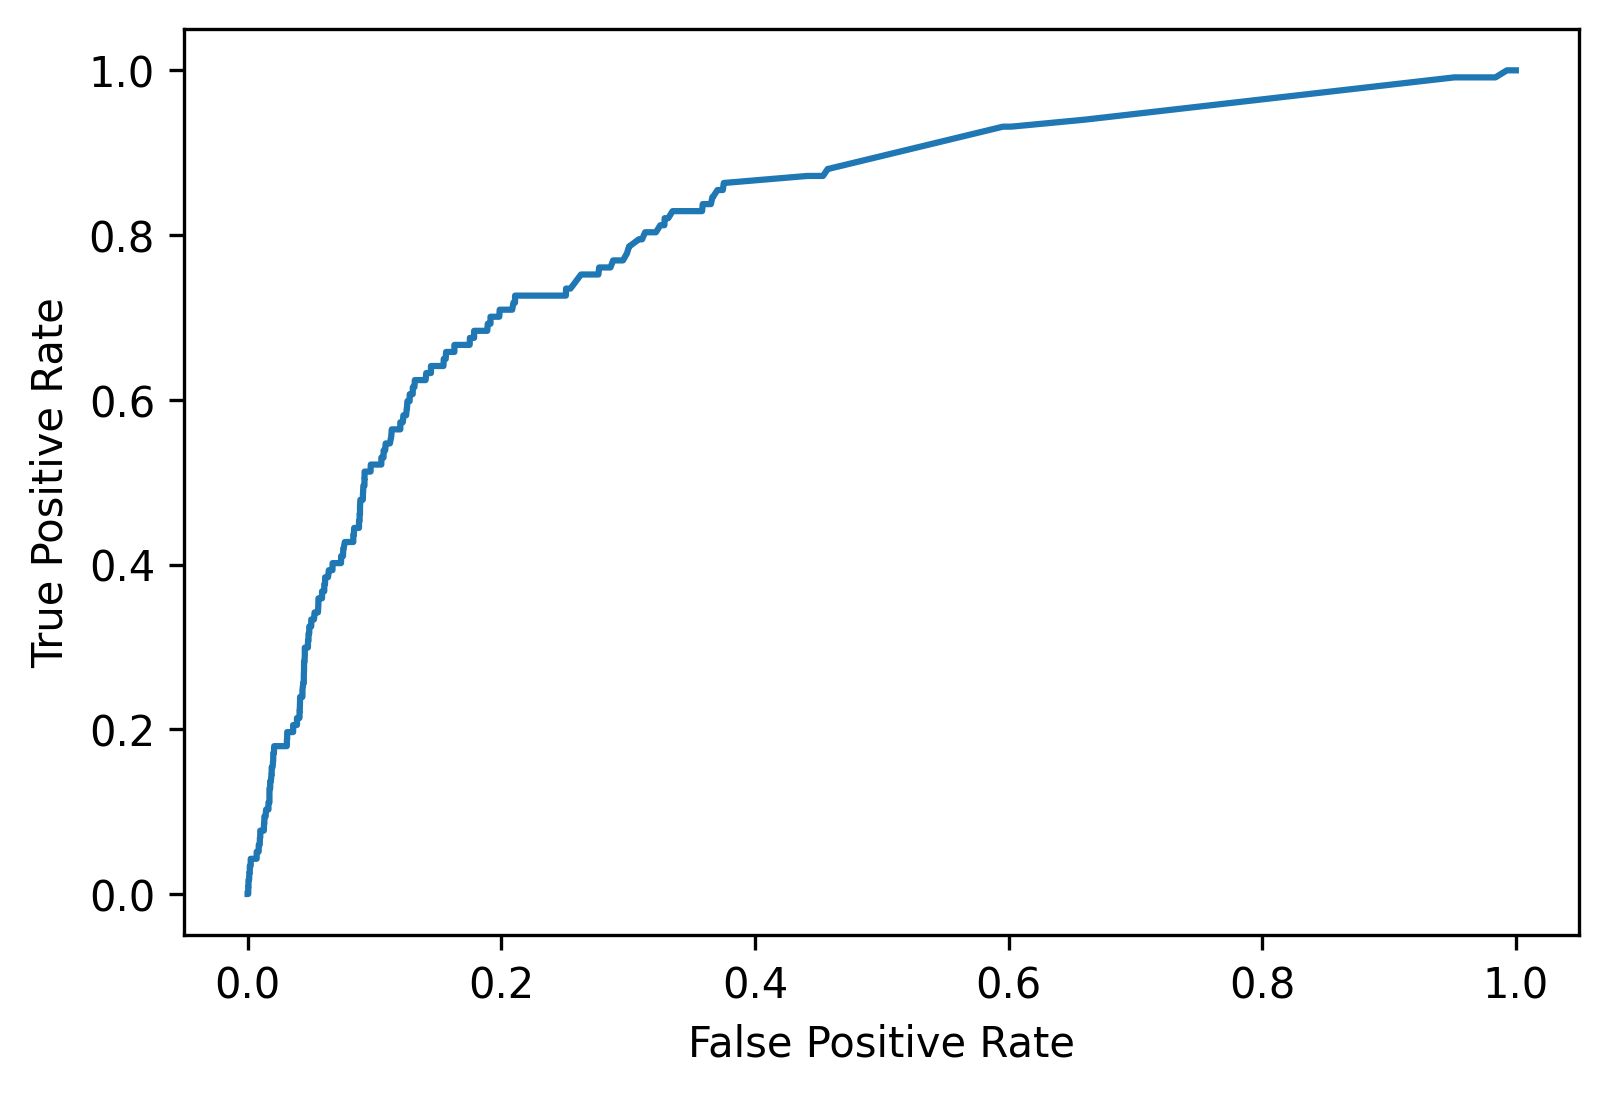
\includegraphics[width=\textwidth]{../images/BiLSTM_test_roc.png}
    \caption{BiLSTM on test}
    \label{fig:BiLSTM_roc_test}
  \end{subfigure}


  \begin{subfigure}[b]{0.32\textwidth}
    \centering
    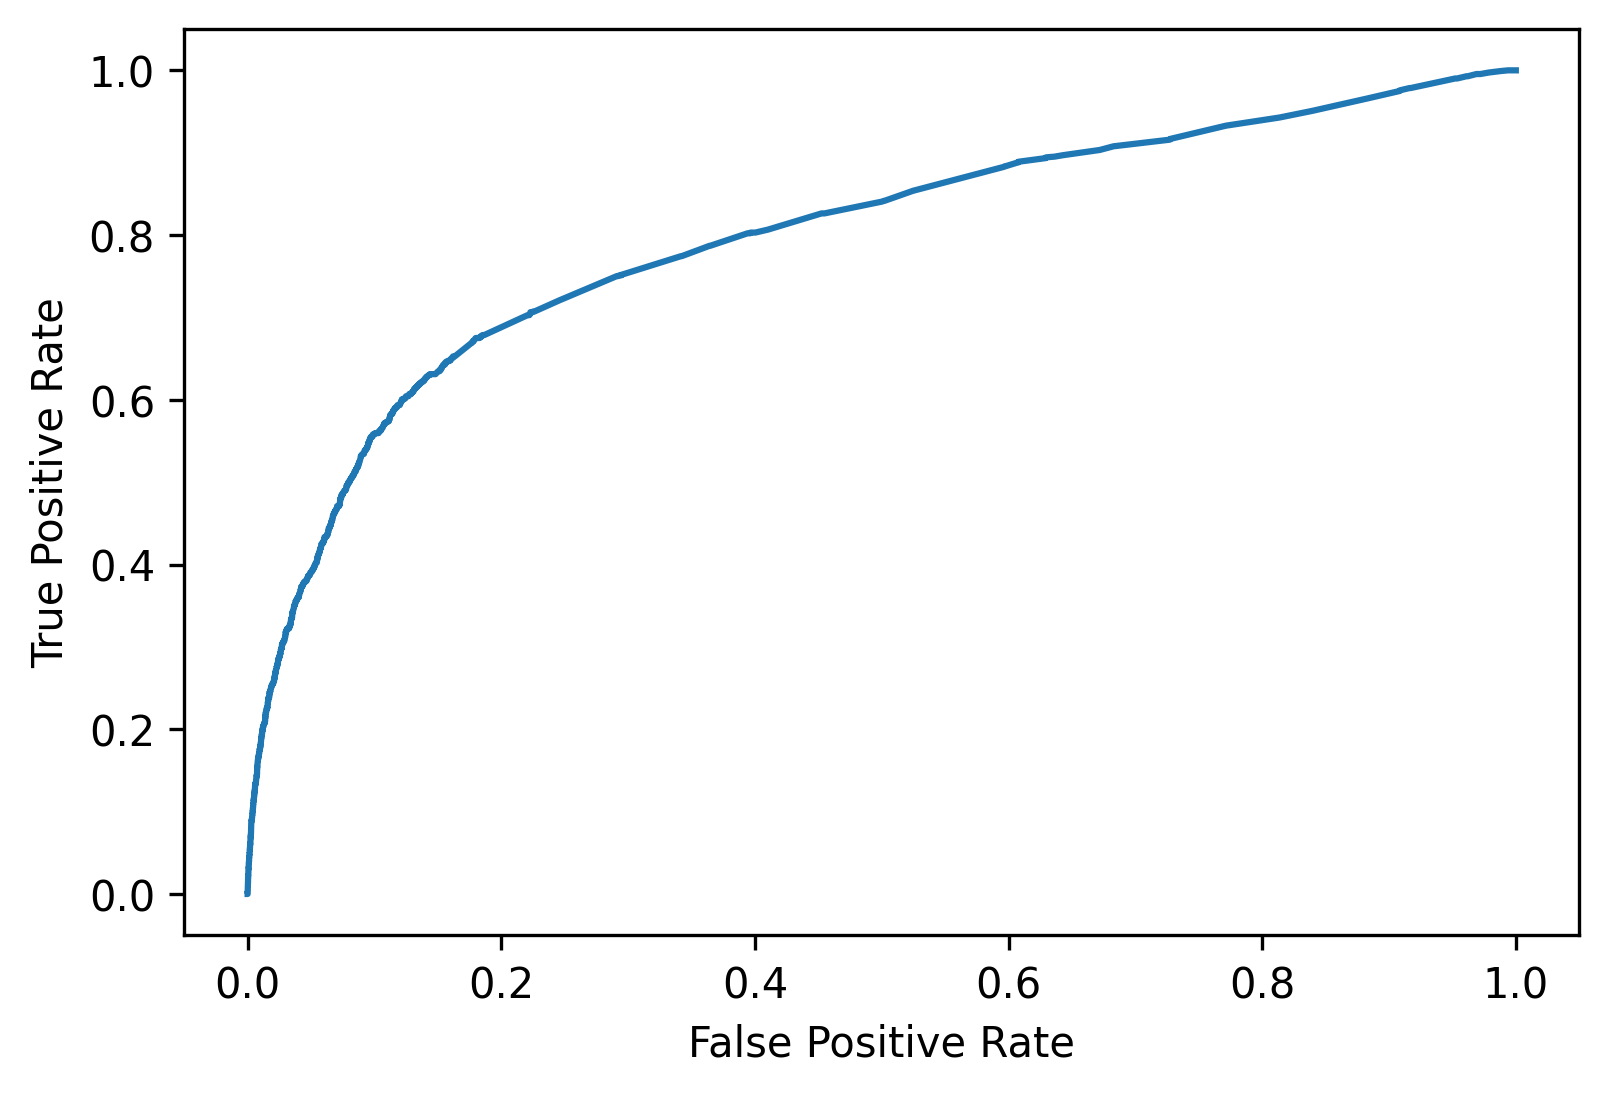
\includegraphics[width=\textwidth]{../images/BiGRU_train_roc.png}
    \caption{BiGRU on train}
    \label{fig:BiGRU_roc_train}
  \end{subfigure}
  \begin{subfigure}[b]{0.32\textwidth}
    \centering
    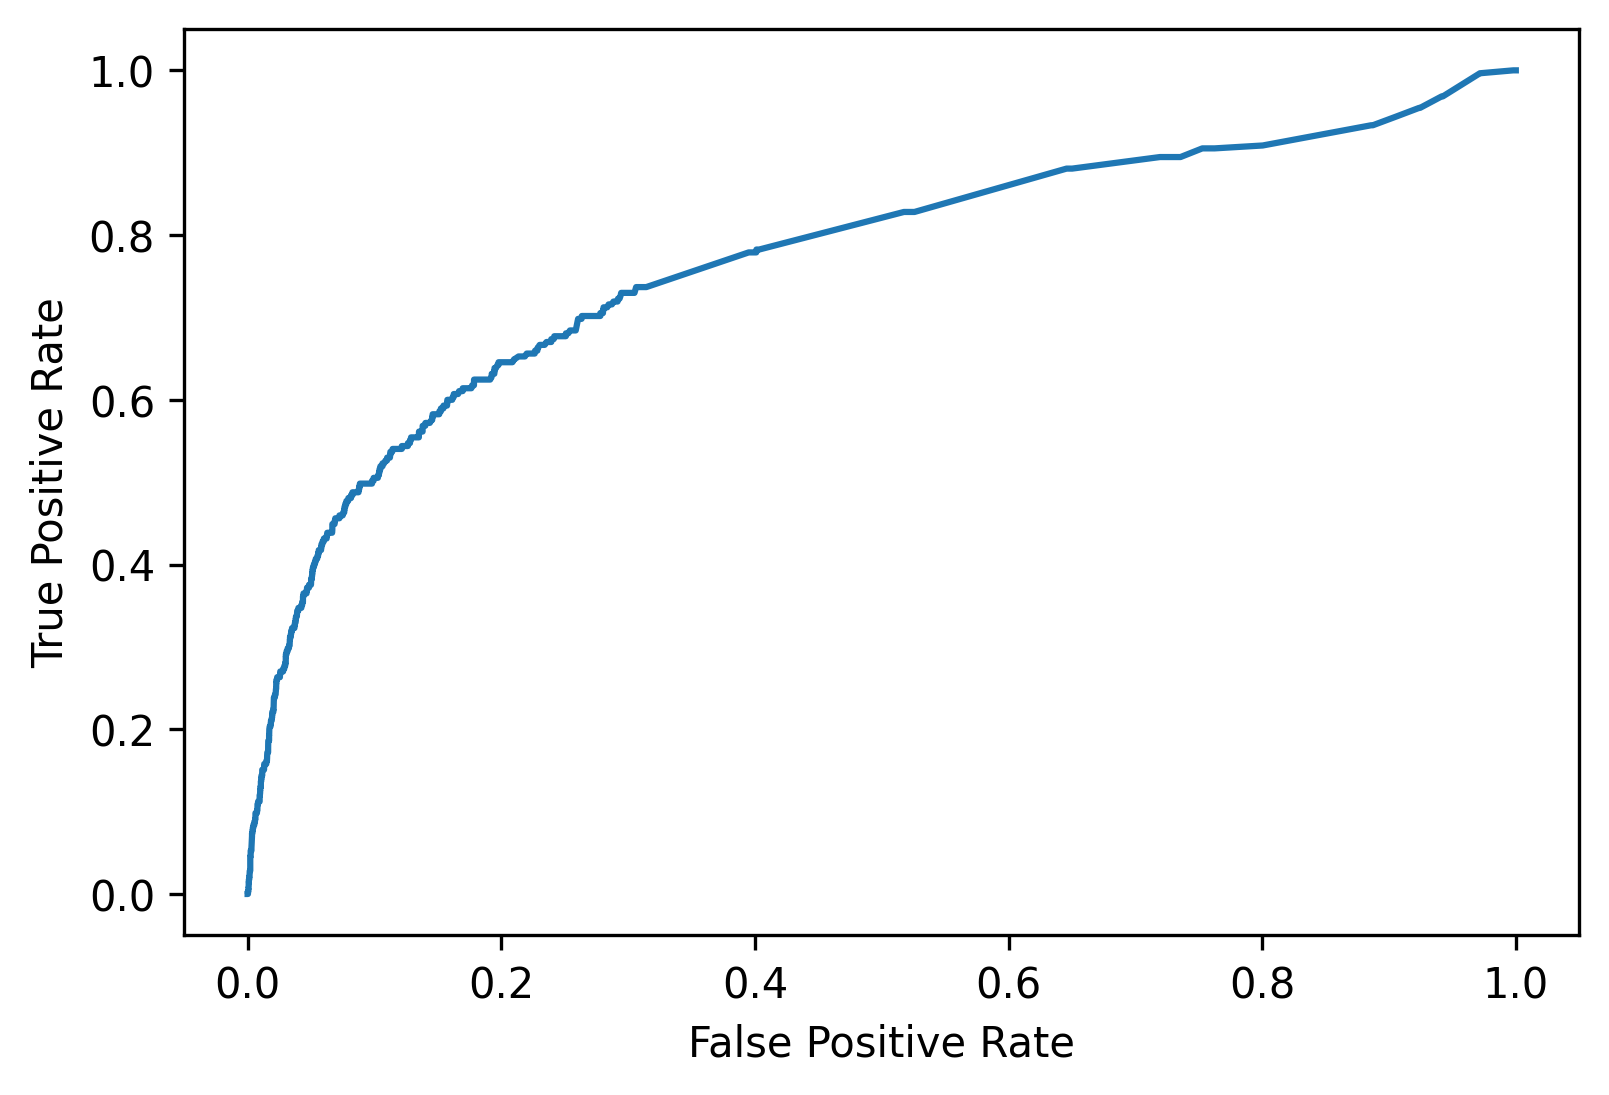
\includegraphics[width=\textwidth]{../images/BiGRU_val_roc.png}
    \caption{BiGRU on validation}
    \label{fig:BiGRU_roc_val}
  \end{subfigure}
  \begin{subfigure}[b]{0.32\textwidth}
    \centering
    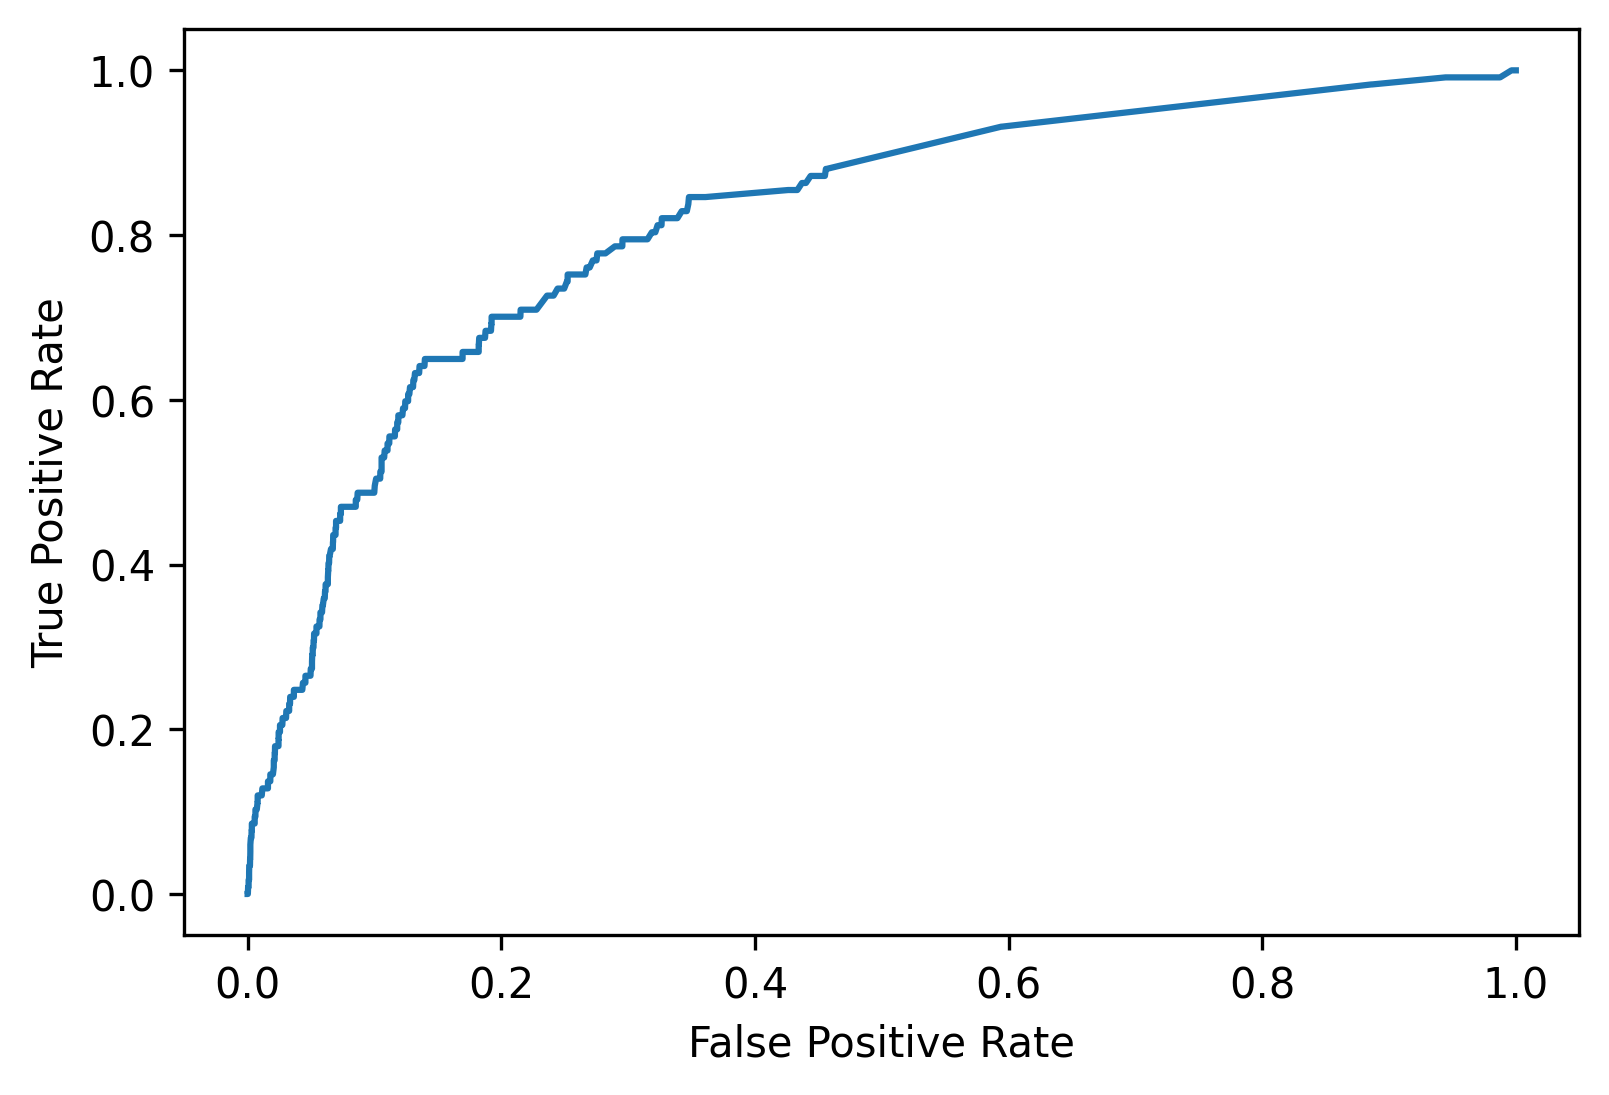
\includegraphics[width=\textwidth]{../images/BiGRU_test_roc.png}
    \caption{BiGRU on test}
    \label{fig:BiGRU_roc_test}
  \end{subfigure}


  \begin{subfigure}[b]{0.32\textwidth}
    \centering
    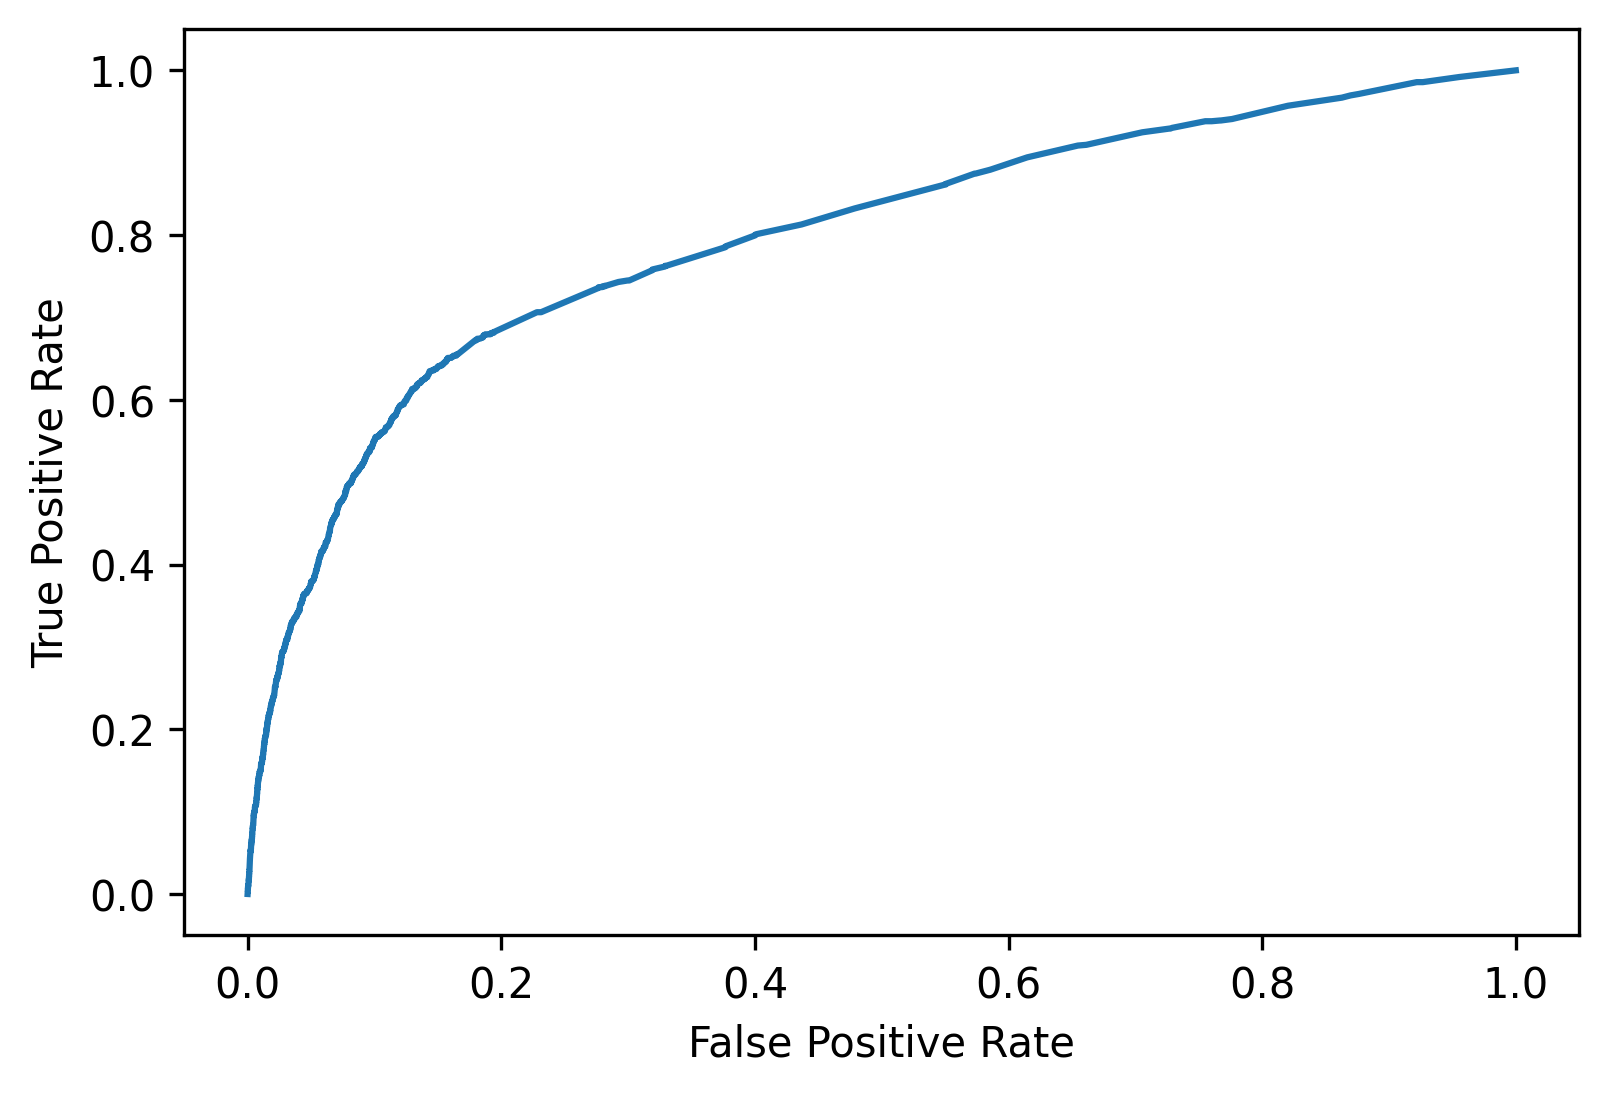
\includegraphics[width=\textwidth]{../images/Transformer_train_roc.png}
    \caption{TEL on train}
    \label{fig:Transformer_roc_train}
  \end{subfigure}
  \begin{subfigure}[b]{0.32\textwidth}
    \centering
    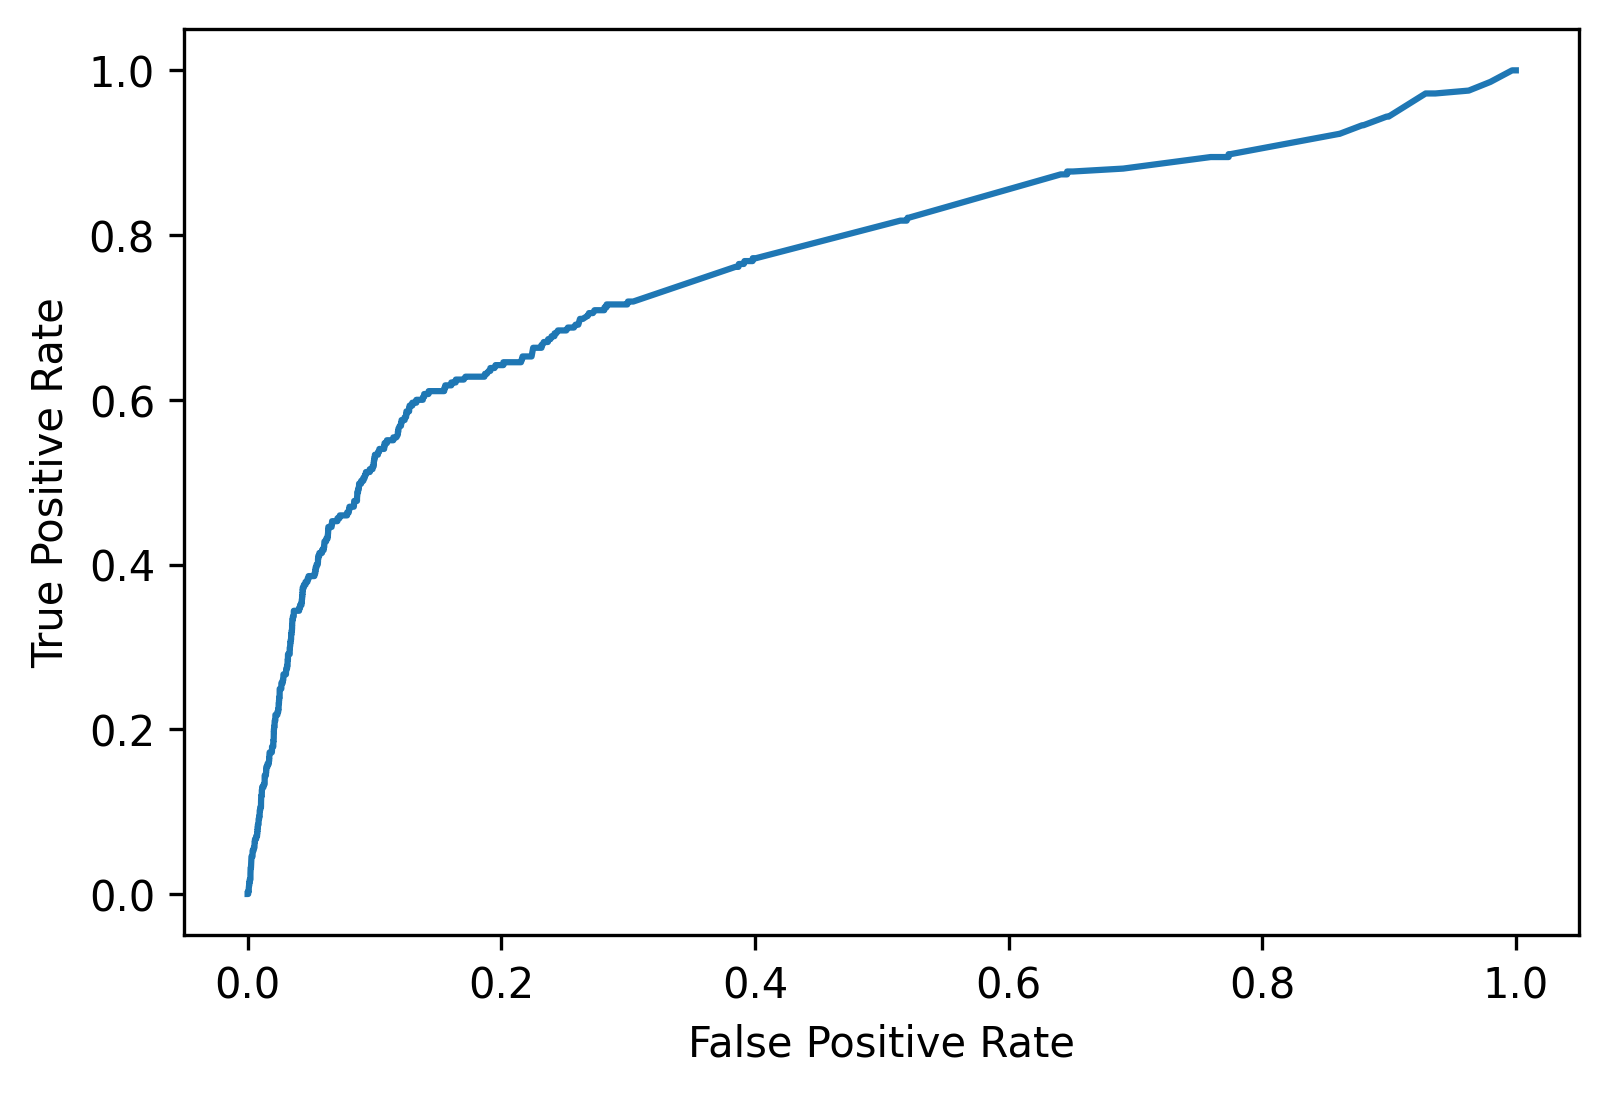
\includegraphics[width=\textwidth]{../images/Transformer_val_roc.png}
    \caption{TEL on validation}
    \label{fig:Transformer_roc_val}
  \end{subfigure}
  \begin{subfigure}[b]{0.32\textwidth}
    \centering
    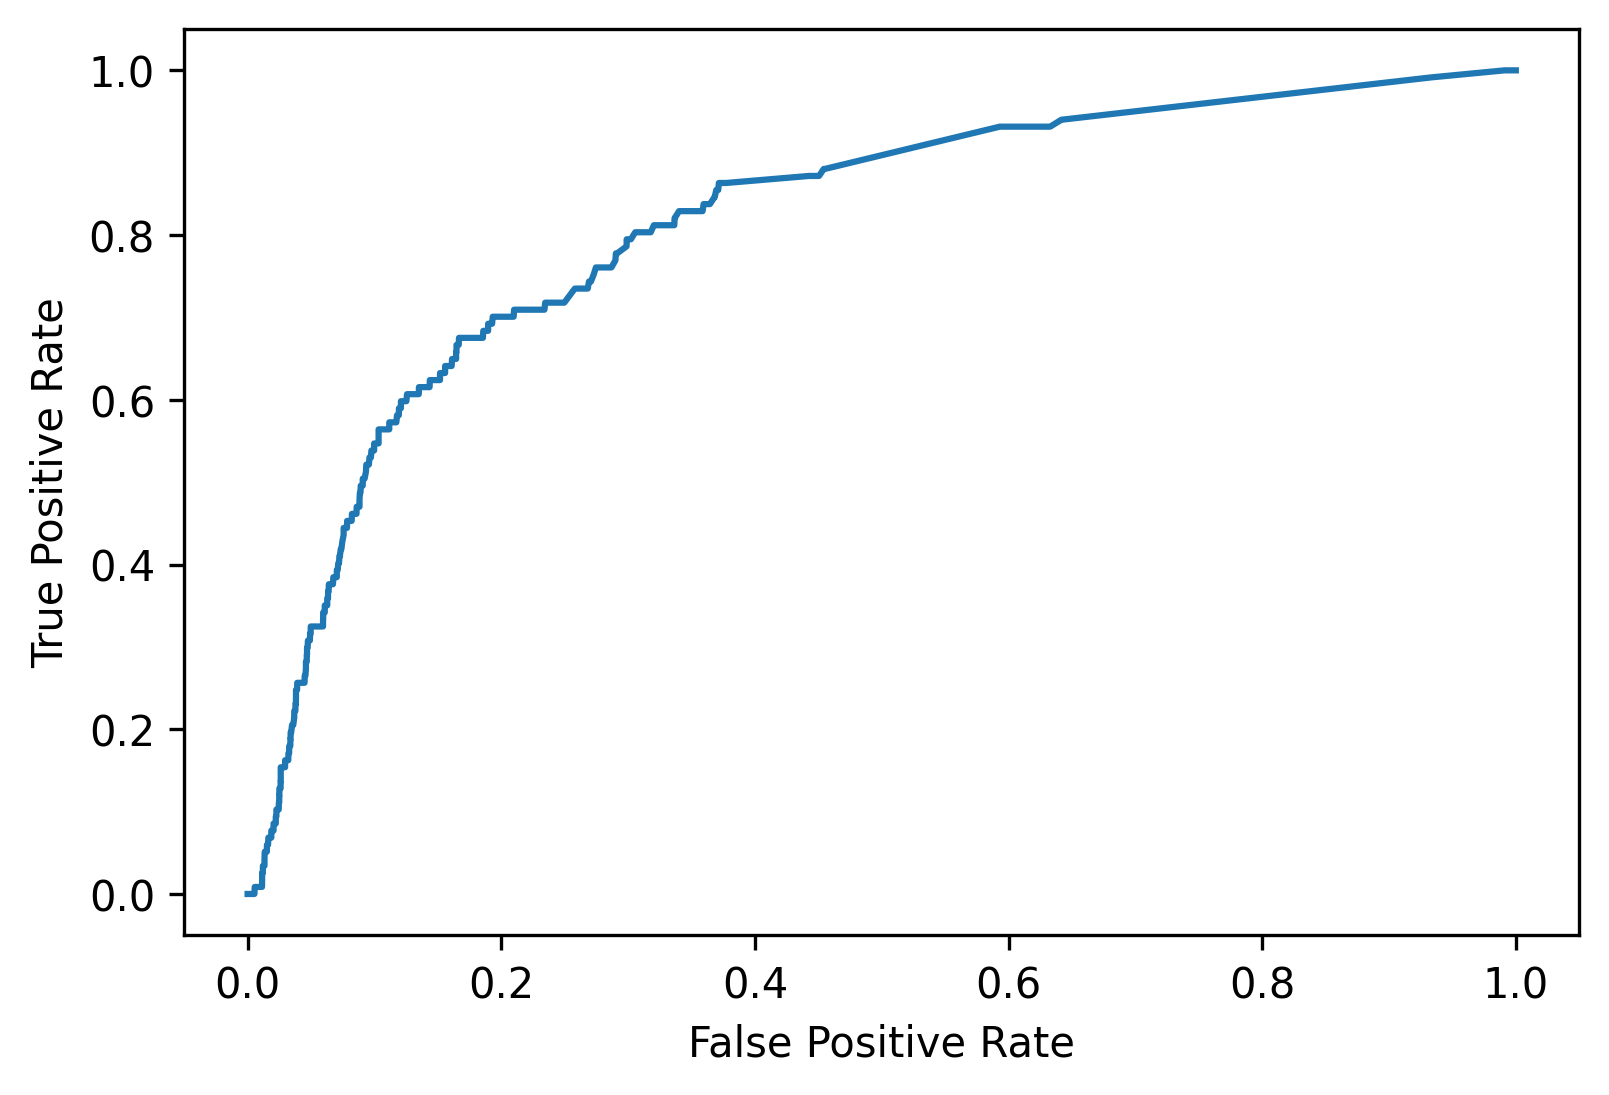
\includegraphics[width=\textwidth]{../images/Transformer_test_roc.png}
    \caption{TEL on test}
    \label{fig:Transformer_roc_test}
  \end{subfigure}

  \caption{receiver operating characteristic curves}
  \label{fig:roc}
\end{figure}

Table~\ref{tab:rocprc} shows the area under curve (AUC) values for PRC and ROC on train, test and validation sets for the 3 models. Comparing the 3 models we find that they are all very similar. However, the BiGRU shows the highest values in the PRC on the test set if that is what we care about. All in all the values are so low though, that these small differences might just be statistical anomalies and could be different in another run of training. We would have thought that the transformer performed better, but it was actually the worst on all datasets when using PRC as the metric.

\begin{table}[ht]
  \centering
  \caption{PRC and ROC AUC values of the 3 models}
  \label{tab:rocprc}
  \begin{tabular}{c|ccc}

           & \multicolumn{3}{c}{ROC}                       \\
           & Train                   & Validation & Test   \\
    \hline
    BiLSTM & 0.7927                  & 0.7673     & 0.8143 \\
    BiGRU  & 0.7962                  & 0.7687     & 0.8161 \\
    TEL    & 0.7963                  & 0.7658     & 0.8135 \\
    \hline
           &                         &            &        \\
           & \multicolumn{3}{c}{PRC}                       \\
           & Train                   & Validation & Test   \\
    \hline
    BiLSTM & 0.0832                  & 0.0529     & 0.0559 \\
    BiGRU  & 0.0902                  & 0.0518     & 0.0675 \\
    TEL    & 0.0745                  & 0.0457     & 0.0455 \\
  \end{tabular}
\end{table}

\subsection{Using a different time window}

In the following we retrain all models with the same configurations but this time we just allow them to learn on a) the past 3 days or b) on the past 5 days in comparison to the 10 days that were used before. As a metric of performance we compare  area under PRC and ROC curve on the test set in Table ~\ref{tab:time_comparison}. The accuracy and confusion matrices have not changed at all, still all models predict all instances to be non-click. More about how this can be addressed in the next section.
From the values in the PRC AUC values in the table it seems like Transformer Encoder Layer and BiGRU have a slightly better test performance when only 3 days are used. For BiLSTM no real difference was visible.

\begin{table}[ht]
  \centering
  \caption{Models trained on different time frames}
  \label{tab:time_comparison}
  \begin{tabular}{c|ccc}
                   & PRC AUC & ROC AUC \\
    \hline
    3 days BiLSTM  & 0.052   & 0.8047  \\
    5 days BiLSTM  & 0.0444  & 0.8098  \\
    10 days BiLSTM & 0.0559  & 0.8143  \\
    \hline
    3 days BiGRU   & 0.0761  & 0.8058  \\
    5 days BiGRU   & 0.0429  & 0.8111  \\
    10 days BiGRU  & 0.0675  & 0.8161  \\
    \hline
    3 days TEL     & 0.0599  & 0.8081  \\
    5 days TEL     & 0.0475  & 0.8121  \\
    10 days TEL    & 0.0455  & 0.8135  \\
  \end{tabular}
\end{table}

\subsection{Dealing with the Data Imbalance}

Until now, we just predicted instances where a model gives a probability of $\leq 0.5$ as "non-click" and otherwise as "click". However, this might not be the best cutoff value. If we look at the ROC curve, we can choose the point on the curve closest to the top-left corner as the best point. We want to achieve a recall (= true positive rate) like in this point. To do so, we can take all our predicted probabilities for instances that are clicks in reality and sort them according to their predicted probability in decreasing order. Let $L$ be the length of that sequence. The element at index $L * recall$ is now the new cutoff probability we will pick for our model. On the training data the optimal cutoff value of around 0.002 to 0.04 was found for a recall of about 0.7 in the ROC curve.
Applying this cutoff to the test data results in new confusion matrices for the models trained on the 10-day sequence as seen in Figure~\ref{fig:confadjusted}. As we see we can now detect more of the clicks but also get a huge amount of false positives.

\begin{figure}[htb]
  \centering
  \begin{subfigure}[b]{0.32\textwidth}
    \centering
    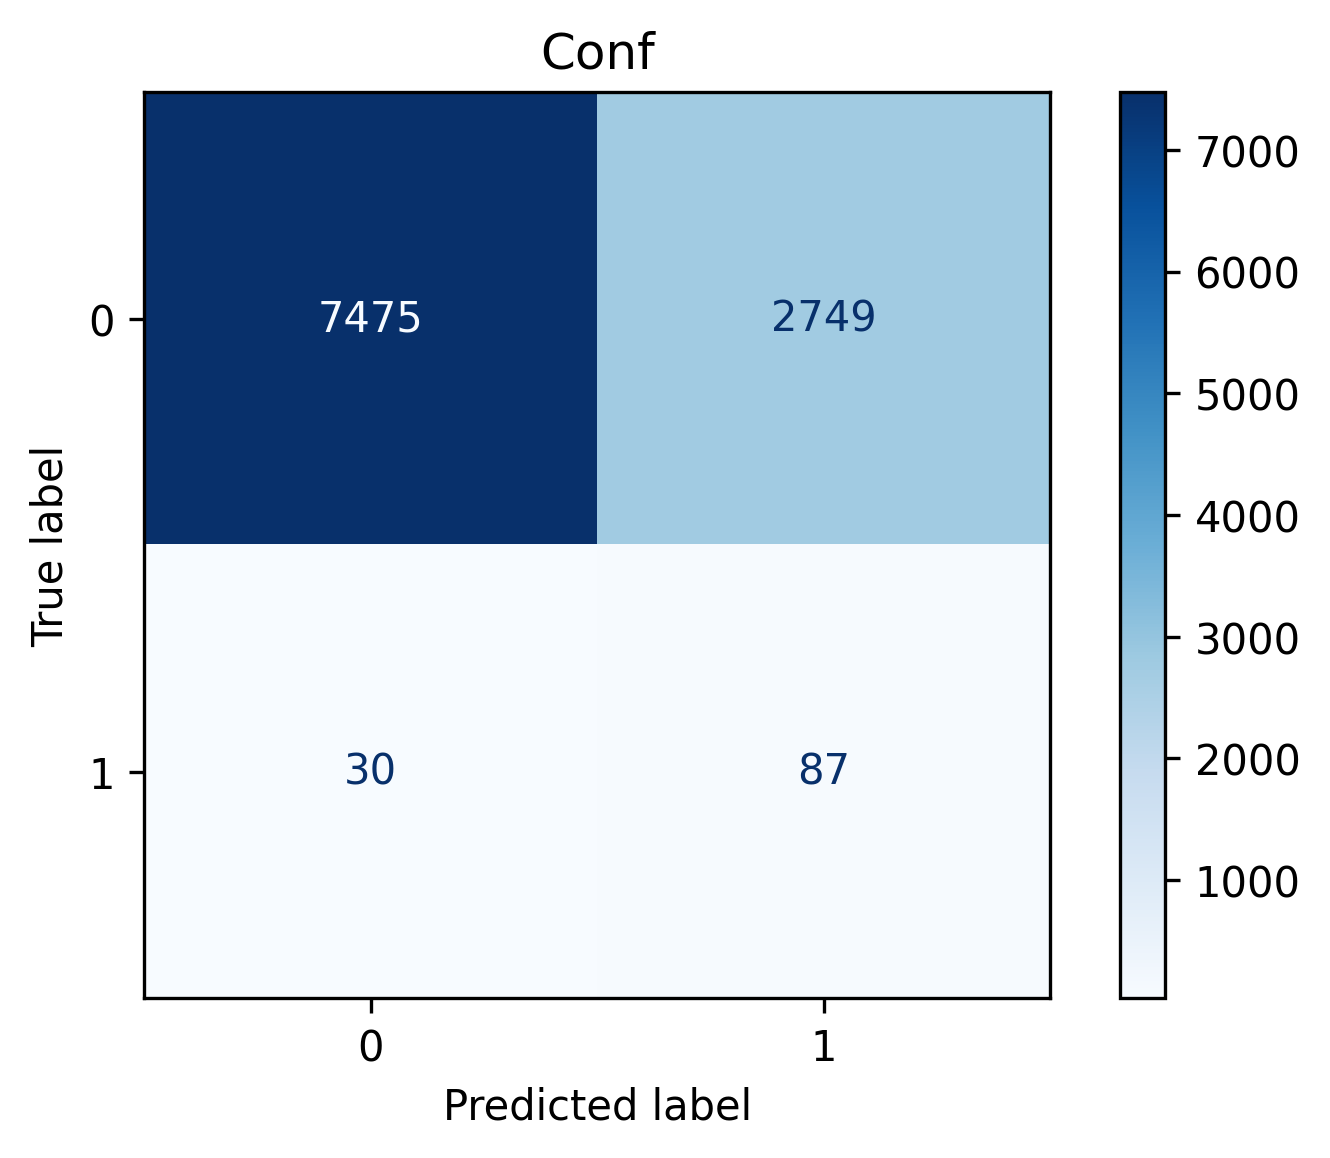
\includegraphics[width=\textwidth]{../images/BiLSTMc_test_conf.png}
    \caption{BiLSTM}
    \label{fig:BiLSTMc_test_conf}
  \end{subfigure}
  \begin{subfigure}[b]{0.32\textwidth}
    \centering
    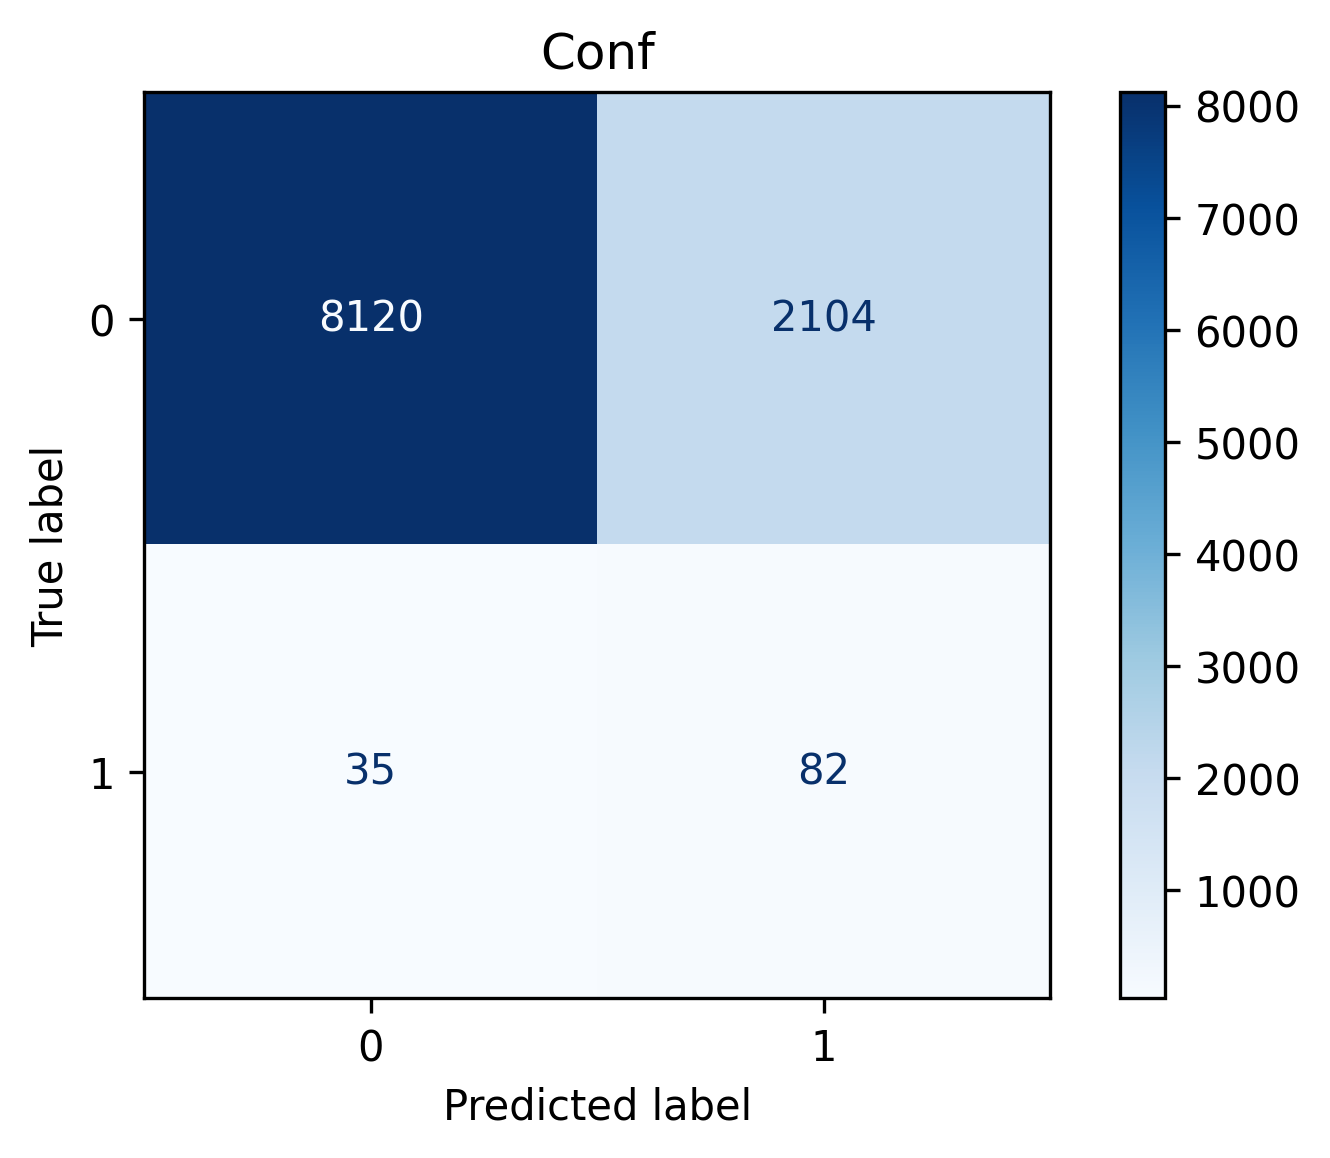
\includegraphics[width=\textwidth]{../images/BiGRUc_test_conf.png}
    \caption{BiGRU}
    \label{fig:BiGRUc_test_conf}
  \end{subfigure}
  \begin{subfigure}[b]{0.32\textwidth}
    \centering
    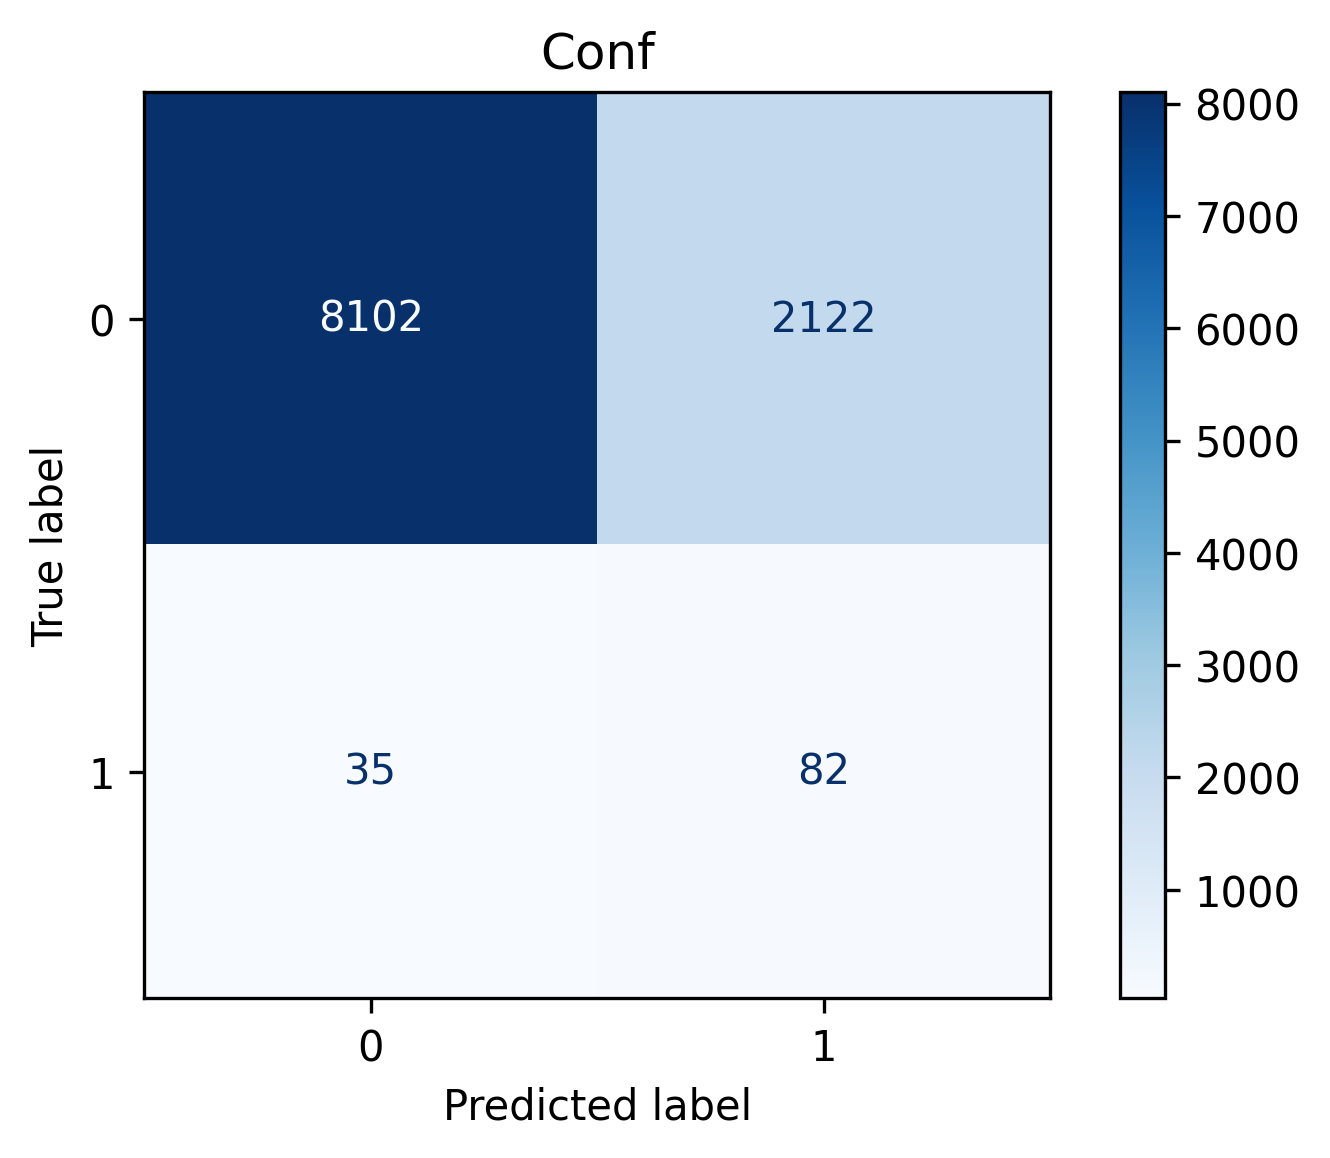
\includegraphics[width=\textwidth]{../images/Transformerc_test_conf.png}
    \caption{TEL}
    \label{fig:Transformerc_test_conf}
  \end{subfigure}

  \caption{Confusion matrices on test data after adjustment of cutoff value}
  \label{fig:confadjusted}
\end{figure}



\section{Discussion}

As the results show it is really hard to have the models produce good results on their own. Because of the imbalance in the data we cannot rely on the raw predictions obtained by minimizing the binary cross entropy during training. If we did so, we would just predict every push notification as a "non-click" right from the get go, which is just not helpful and does not leverage the real power of machine learning. There are other ways however to deal with this imbalance, not shown in this report. For example, we could perform over- or undersampling.
A real improvement could be found in the way we selected our features.
For example one of the strongest predictors of future clicks might be past clicks. I suppose we could build a more powerful model just by utilizing the sequence of past clicks (click vs. non-click) and maybe the time of the day alone. This would however not be very useful in the general setting that we want to design interesting push notifications, but only in specific cases where the model would decide for a particular user if it makes sense to send the push notification or not.
Another interesting feature would be time of the day. For example is it likely that people tend to click push notifications with different topics depending on if they are at work or in their leisure time. Also, comparisons with baseline models would be useful which was not done in this report.

% \newpage
% \addcontentsline{toc}{section}{Bibliography}
% \renewcommand\refname{Bibliography}
% \bibliographystyle{plainnat}
% \bibliography{references}
\end{document}
